{
    \chapter{Zufallsvariable}\index{Zufallsvariable|(}

    \section{Motivation und Einführung}\index{Zufallsvariable!Beschreibung|(}

    Bisher hat uns immer direkt das Ergebnis eines Elementarereignisses
    interessiert, zum Beispiel haben wir uns gefragt, wie wahrscheinlich es
    ist, dass eine Münze Kopf zeigt oder eine Drei gewürfelt wird. Nun
    interessiert uns aber nicht mehr das Elementarereignis, sondern die
    {\quotedblbase}Informationen{\textquotedblleft}, die aus mehreren
    Elementarereignissen entstehen. Am Einfachsten ist das mit einem
    Beispiel verständlich. 

    \begin{bsp}\label{bsp:muenze}
    Der Dozent bietet uns folgendes Spiel an: Jeder Student zahlt dem
    Dozenten 20 Cent Einsatz und wirft dann 3 Münzen. 
    
    Bei den Münzen wird
    {\quotedblbase}Kopf${\triangleq}K${\textquotedblleft} oder
    {\quotedblbase}Zahl${\triangleq}Z${\textquotedblleft} registriert. Je
    nach der Anzahl der geworfenen {\quotedblbase}Köpfe{\textquotedblleft}
    zahlt der Dozent anschließend die Beträge in Tabelle \ref{tab:auszahlungen}\\

    Wie wahrscheinlich sind die einzelnen Auszahlungen? Was muss der Dozent
    im Schnitt zahlen? Ist das Spiel fair? 
    
    Für die kürzere Schreibweise führen wir ein:

    \[X_{i}...\text{Anzahl der vom }i\text{-ten Studenten bei 3 Versuchen geworfene Köpfe}\]
    \[Y_{i}...\text{Auszahlung an den }i\text{-ten Studenten}\]

    Wir betrachten den ersten Studenten:

    Dieser wirft 2 {\quotedblbase}Köpfe{\textquotedblleft}, also ist $X_{1}=2$.

    Aber was heißt das und was ist der Unterschied zwischen $X_{1}$ und $X_{1}=2$?

    \begin{center}
    \begin{tabular}{c|c}
    \hline
    \textbf{Zufallsvariable} & \textbf{Realisation von $X_1$}\\
    \hline
     $X_1$ & $X_1=2$\\
     \parbox[t]{0.33\linewidth}{Symbolische Kurzbeschreibung des Münzspiels} 
            & \parbox[t]{0.33\linewidth}{Die Realisation $2$ ist eingetreten.}\\
     \hline
    \end{tabular}
    \end{center}

    Nun stellen wir uns natürlich die Frage, wie Wahrscheinlich der Student
    zweimal Kopf würfelt. Dafür betrachten wir zuerst die Grundmenge $\Omega$, also die Menge, die alle
    möglichen Ausgänge des Spiels beinhaltet:
    \[\Omega=\{ZZZ,KZZ,ZKZ,ZZK,KKZ,KZK,ZKK,KKK\}\]
    Wir gehen von einer fairen Münze aus, es gilt: $\mathbb P\left(Z\right)=\mathbb P\left(K\right)=\frac{1}{2}$.
    Zusätzlich wissen wir aus dem vorherigen Kapitel, dass wenn die
    Ereignisse total unabhängig sind, sich jede Wahrscheinlichkeit, zum Beispiel $\mathbb P\left(ZKZ\right)$,
    leicht berechnen lässt:
    \[\mathbb P\left(ZKZ\right)=\mathbb P(Z)\mathbb P\left(K\right)\mathbb P\left(Z\right)=\frac{1}{2}\cdot\frac{1}{2}\cdot\frac{1}{2}=\frac{1}{8}\]

    Das gilt trivialerweise auch für die anderen Ausgänge des Spiels. Und was macht die 
    Zufallsvariable $X_{1}$ genau? Sie {\quotedblbase}bewertet{\textquotedblleft} die 
    Elemente der Grundmenge $\Omega $ anhand der Anzahl von {\quotedblbase}Köpfen{\textquotedblleft}:
    \begin{eqnarray*}
        X_{1}\left(ZZZ\right)&=&0\\
        X_{1}\left(KZZ\right)=X_{1}\left(ZKZ\right)=X_{1}\left(ZZK\right)&=&1\\
        X_{1}\left(KKZ\right)=X_{1}\left(KZK\right)=X_{1}\left(ZKK\right)&=&2\\
        X_{1}\left(KKK\right)&=&3
    \end{eqnarray*}
    Mathematisch ausgedrückt ist eine Zufallsvariable eine Abbildung der Grundmenge $\Omega$ 
    in die reellen Zahlen:

    \[
    X_{1}:\Omega \rightarrow \mathbb R
    \]
    Diese Abbildung ist nicht bijektiv, wie sich mit Tabelle \ref{tab:zv_abbildungen} leicht nachprüfen lässt:\\

    Offensichtlich existieren jeweils drei Ereignisse, die auf 1 bzw. 2
    abbilden und somit ist die Abbildung nicht eindeutig umkehrbar.
    

    Anmerkung: für  $\mathbb P\left(X_{1}=1\right)$ bzw. $\mathbb P\left(X_{1}=2\right)$
    wurden die einzelnen Wahrscheinlichkeiten einfach addiert, da sich die Ereignisse paarweise
    ausschließen.
    \end{bsp}

    \begin{table}
        \centering
        \begin{tabular}{cc}
        \hline
        \textbf{Anzahl der Köpfe} & \textbf{Auszahlung in Cent}\\
        \hline
         0 & 0\\
         1 & 0\\
         2 & 20\\
         3 & 100\\
         \hline
        \end{tabular}
        \caption{Auszahlungsbeträge bei 3 Münzwürfen}\label{tab:auszahlungen}
    \end{table}

    \begin{table}
        \centering
        \begin{tabular}{ccc}
        \hline
        \textbf{Ereignisse} & \textbf{Realisationen von $X_1$}& \textbf{Wahrscheinlichkeit $P_1$}\\
        \hline
         $\{ZZZ\}$ & 0 & $\mathbb{P}(X_1=0)=\frac{1}{8}$\\
         $\{KZZ,ZKZ,KZZ\}$ & 1 & $\mathbb{P}(X_1=0)=\frac{3}{8}$\\
         $\{KKZ,KZK,ZKK\}$ & 2 & $\mathbb{P}(X_1=0)=\frac{3}{8}$\\
         $\{KKK\}$ & 3 & $\mathbb{P}(X_1=0)=\frac{1}{8}$\\
         \hline
        \end{tabular}
        \caption{Abbildungen der Ereignisse in Wahrscheinlichkeiten ($\Omega\to\mathbb R$)}\label{tab:zv_abbildungen}
    \end{table}
    \index{Zufallsvariable!Beschreibung|)}

    \section{Mathematische Definition}\index{Zufallsvariable!Mathematische Definition|(}

    Die Wahrscheinlichkeit des im vorherigen Kapitel (Siehe Definition \ref{def:axiome_kolmogorov}) beschrieben
    Wahrscheinlichkeitsraumes  $\left(\Omega,\mathcal S,\mathbb P\right)$ wird mithilfe von $X$ auf einen
    neuen Wahrscheinlichkeitsraum abgebildet.

    \[\left(\Omega ,\mathcal S,\mathbb P\right)\Rightarrow X\Rightarrow (\mathcal B,\mathcal F,\mathbb P_{X})\]
    Dem Ereignis $F\in \mathcal F$ ordnen wir nun die Wahrscheinlichkeit seiner {\quotedblbase}Verursacher{\textquotedblleft} zu:

    \[
    \mathbb P_{X}\left(F\right)=
    \mathbb P(X\in F)=\mathbb P\left(X^{-1}\left(F\right)\right)=
    \mathbb P\left(\{\omega:X\left(\omega \right)\in F\}\right)
    \]

    \begin{definition}
    Das \textbf{Wahrscheinlichkeitsmaß}\index{Wahrscheinlichkeitsmaß} $\mathbb P_{X}$ heißt das zu X gehörige \textbf{Bildmaß}.\index{Bildmaß}
    Vereinfacht kann $X$ auch als Abbildung 
    \[
    X:\Omega\rightarrow \mathbb R^{d}
    \]  
    definiert werden. Dabei gilt:

    \begin{itemize}
    \item wenn $\Omega$ überabzählbar ist, muss man von $X$ die Eigenschaft 
        \quotedblbase Messbarkeit\textquotedblleft verlangen.
    \item meistens ist $d=1$, bei $d>1$ wird $X=\left(X_{1},...,X_{d}\right)$ ein Vektor von reellen
        Zufallsvariablen.
    \end{itemize}
    \end{definition}

    \begin{bsp}\label{bsp:abbildung_wahrscheinlichkeitsraum} \textbf{anhand des Münzbeispiels (siehe Beispiel \ref{bsp:muenze})}\\
        \begin{itemize}
            \item $\Omega\;\Rightarrow\;\mathcal B$
                \[\{ZZZ,KZZ,ZKZ,ZZK,KKZ,KZK,ZKK,KKK\}\;\Rightarrow\;\{0,1,2,3\}\]
            \item $\mathcal S\;\Rightarrow\;\mathcal F$\\
                Abhängig von der Anforderung
            \item $\mathbb P\;\Rightarrow\;\mathbb P_X$
                \[\forall \omega \in \Omega :\mathbb P\left(\omega \right)=\frac{1}{8}\Rightarrow
                    \begin{cases}\mathbb P_{X_1}\left(0\right)=\mathbb P_{X_1}\left(3\right)=\frac{1}{8}\\
                    \mathbb P_{X_1}\left(1\right)=\mathbb P_{X_1}\left(2\right)=\frac{3}{8}
                    \end{cases}\]
        \end{itemize}

        \textbf{Graphische Erklärung}\\
        Alle Elementarereignisse  $\omega \in \Omega$, also
        die durch Zufall eingetretene Ereignisse (z.B. $\{ZZZ\},\{KZK\},\{KKK\}$),
        werden über die Abbildung der Zufallsvariable $X$ auf die reellen Zahlen
        und in die Menge $\mathcal B$
        abgebildet, dem Ereignis wird eine Realisation zugeordnet. 

        Abbildung \ref{fig:abbildung_wahrscheinlichkeitsraum} beschreibt das komplette System anschaulich: 
        
        Die blauen Bereiche repräsentieren eine Abbildung, die Quadrate einen
        vollständigen Wahrscheinlichkeitsbereich.

    \end{bsp}

    \begin{figure}
    \centering
        \includegraphics[width=5.8102in,height=7.8744in]{chapters/zufallsvariable/wahrscheinlichkeitsraum}
        \caption{Abbildung des Wahrscheinlichkeitsraumes von $X$ (siehe Beispiel \ref{bsp:abbildung_wahrscheinlichkeitsraum})}
        \label{fig:abbildung_wahrscheinlichkeitsraum}
    \end{figure}

    \index{Zufallsvariable!Mathematische Definition|)}
    \section{Diskrete Zufallsvariable}\index{Diskrete Zufallsvariable|(}\index{Zufallsvariable!diskret|see{Diskrete Zufallsvariable}}

    \begin{figure}
    \centering
        \begin{tikzpicture}
            {
    \begin{axis}[domain=0:8,
            axis x line=bottom, % no box around the plot, only x and y axis
            axis y line=left, % the * would suppress the arrow tips
            xlabel=Anzahl der Köpfe,
            ylabel=Wahrscheinlichkeit $p$,
            legend style={at={(1.05,0.75)}},
            xtick={0,1,...,4},
            %legend pos=south east,
            samples=50,
            height=6cm,
            width=10cm,
            clip=false]
            \def\pvala{0.125}
            \def\pvalb{0.375}
            \def\pvalc{0.375}
            \def\pvald{0.125}

            %calc missing values
            \pgfmathsetmacro{\tvala}{\pvala}
            \pgfmathsetmacro{\tvalb}{\pvala+\pvalb}
            \pgfmathsetmacro{\tvalc}{\pvala+\pvalb+\pvalc}
            \pgfmathsetmacro{\tvald}{\pvala+\pvalb+\pvalc+\pvald}

            \addplot[blue] coordinates{(-1,0)(0,0)};
            \addlegendentry[align=left]{Verteilungsfunktion};%TODO: add a better label
            \addplot[blue,forget plot] coordinates{(0,\tvala)(1,\tvala)};
            \addplot[blue,forget plot] coordinates{(1,\tvalb)(2,\tvalb)};
            \addplot[blue,forget plot] coordinates{(2,\tvalc)(3,\tvalc)};
            \addplot[blue,forget plot] coordinates{(3,1)(5,1)};

            \draw[dotted] (axis cs:0,0) -- (axis cs:0,\tvala);
            \draw[dotted] (axis cs:1,\tvala) -- (axis cs:1,\tvalb);
            \draw[dotted] (axis cs:2,\tvalb) -- (axis cs:2,\tvalc);
            \draw[dotted] (axis cs:3,\tvalc) -- (axis cs:3,1);
            %\draw[dotted] (axis cs:4,\tvald) -- (axis cs:4,1);

            \addplot[discontinuityblue,forget plot] coordinates{(0,0)
                    (1,\tvala)
                    (2,\tvalb)
                    (3,\tvalc)};
            \addplot[continuityblue,forget plot] coordinates{(0,\tvala)
                    (1,\tvalb)
                    (2,\tvalc)
                    (3,1)};

            \addplot[red] coordinates{(-1,0)(0,0)};
            \addlegendentry[align=left]{Wahrsch.verteilung};%TODO: add better label
            \addplot[red,forget plot] coordinates{(0,\pvala)(1,\pvala)};
            \addplot[red,forget plot] coordinates{(1,\pvalb)(2,\pvalb)};
            \addplot[red,forget plot] coordinates{(2,\pvalc)(3,\pvalc)};
            \addplot[red,forget plot] coordinates{(3,\pvald)(4,\pvald)};
            \addplot[red,forget plot] coordinates{(4,0)(5,0)};

            \draw[dotted] (axis cs:0,0) -- (axis cs:0,\pvala);
            \draw[dotted] (axis cs:1,\pvala) -- (axis cs:1,\pvalb);
            %\draw[dotted] (axis cs:2,\pvalb) -- (axis cs:2,\pvalc);
            \draw[dotted] (axis cs:3,\pvalc) -- (axis cs:3,\pvald);
            \draw[dotted] (axis cs:4,\pvald) -- (axis cs:4,0);

            \addplot[discontinuityred,forget plot] coordinates{(0,0)
                    (1,\pvala)
                    %(2,\pvalb)
                    (3,\pvalc)
                    (4,\pvald)};
            \addplot[continuityred,forget plot] coordinates{(0,\pvala)
                    (1,\pvalb)
                    %(2,\pvalc)
                    (3,\pvald)
                    (4,0)};
    \end{axis}
}

        \end{tikzpicture}
        \caption{die diskrete Verteilungsfunktion und die diskrete Wahrscheinlichkeitsverteilung von Beispiel \ref{bsp:muenze}}.
        \label{fig:diskrete_verteilung_funktion}
    \end{figure}

    \subsection{Verteilungsfunktion\index{Verteilungsfunktion!diskret|see{diskrete Verteilungsfunktion}}\index{diskrete Verteilungsfunktion} einer diskreten Zufallsvariable}

    Eine diskrete Zufallsvariable X besitzt endlich oder abzählbar unendlich viele Realisationen
    $x_{i},$ die mit Wahrscheinlichkeit $p_{i}=\mathbb P\left(X=x_{i}\right)>0$ angenommen werden. 
    Für jedes $x\in\mathbb R$ ist die Verteilungsfunktion (siehe Abbildung \ref{fig:diskrete_verteilung_funktion} die blaue Line) $F_{X}:\mathbb R\rightarrow [0,1]$
    der Zufallsvariablen $X$ definiert durch:

    \[
    F_{X}\left(x\right)=\mathbb P(X\le x)
    \]
    Die Verteilungsfunktion ist somit monoton steigend und immer zwischen $0$ und $1$. Für jeden Wert
    $F_{X}\left(x_{i}\right)$ an der Stelle $i$ gilt:

    \[
        F_{X}\left(x_{i}\right)=\sum _{j=1}^{i}p_{j}=
        \sum_{j=1}^{i}{\mathbb P\left(X=x_{j}\right)}
    \]

    \subsection{Wahrscheinlichkeitsverteilung\index{Wahrscheinlichkeitsverteilung!diskret|see{diskrete Wahrscheinlichkeitsverteilung}}\index{diskrete Wahrscheinlichkeitsverteilung}
        einer diskreten Zufallsvariable}
    Siehe Abbildung \ref{fig:diskrete_verteilung_funktion} die rote Line.

    Eine diskrete Zufallsvariable $X$ besitzt endlich oder abzählbar unendlich
    viele Realisationen $x_{i},$ die mit Wahrscheinlichkeit $p_{i}=\mathbb P\left(X=x_{i}\right)>0$
    angenommen werden. Für diese $x_{i}$ gilt: 

    \[\sum _{i=1}^{{\infty}}{\mathbb P\left(X=x_{i}\right)}=1\]

    Die Angabe aller $p_{i},i=1,...,{\infty}$ heißt die Dichte von $X$.

    \subsection{Gemeinsame Verteilung zweier diskreter Zufallsvariablen}\index{Gemeinsame Verteilung!diskreter Zufallsvariablen}
    \begin{bsp}\label{bsp:muenze_3}Dafür erweitern wir unser Münzspiel(Beispiel \ref{bsp:muenze}) um folgende Annahme: 

    Es würfelt ein zweiter Student und wir führen
    dafür die Zufallsvariable $X_{2}$ ein. Den Dozent interessiert aber nur, wie viel er insgesamt auszahlen
    muss. Zu Beginn haben wir gesagt:

    \begin{center}
    \begin{tabular}{ccccc}
    \textbf{Kopfanzahl} & 0 & 1 & 2 & 3\\
    \hline
    \textbf{Auszahlung [Cent]} & 0 & 0 & 20 & 100
    \end{tabular}
    \end{center}

    Da uns nur noch der Auszahlungsbetrag interessiert führen wir eine neue Zufallsvariable $Y$ ein.
    \[Y_i...\text{Auszahlungsbetrag an den }i\text{-ten Studenten.}\]
    Nun können wir für zwei Studenten mit $Y_{1}$ und $Y_{2}$ die Auszahlungssumme $S_{2}=Y_{1}+Y_{2}$ definieren 
    (siehe Tabelle \ref{tab:auszahlung_2_studenten})

    Anstatt den Auszahlungsbeträgen ist es für den Dozenten viel wichtiger,
    wie wahrscheinlich er diese Beträge auszahlen muss. Wir haben also eine
    Auszahlungswahrscheinlichkeit von Paaren:

    \[\mathbb P_{Y_{1}Y_{2}}\left(y_{1},y_{2}\right)=\mathbb P\left(Y_{1}=y_{1},Y_{2}=y_{2}\right)\]

    Da diese zwei Zufallsvariablen voneinander unabhängig sind (genauere Definition folgt später), kann %TODO: später ersetzen durch referenz
    die Tabelle \ref{tab:auszahlungswahrscheinlichkeit_2_studenten} mit der Eigenschaft
    $\mathbb P_{Y_{1}Y_{2}}\left(y_{1},y_{2}\right)=\mathbb P_{1}\left(y_{1}\right)\mathbb P_{2}(y_{2})$
    berechnet werden.

    Hat man nur diese Tabelle und man
    möchte die Verteilung $\mathbb P_{1}\left(y_{1}\right)$ berechnen, dann geschieht das mit:

    \[
    \mathbb P_{1}\left(y_{1}\right)=\sum_{y_2}{\mathbb P_{Y_{1}Y_{2}}(y_{1},y_{2})}
    \]
    Das ist nichts anderes als die Spalten- bzw. Zeilensumme. 

    \end{bsp}

    \begin{table}
        \centering
        \begin{tabular}{c|ccc}
        \hline
        \textbf{Summe $S_2$} & $Y_1=0$ & $Y_2=20$ & $Y_3=100$\\
        \hline
         $Y_2=0$ & 0 & 20 & 100\\
         \hline
         $Y_2=20$ & 20 & 40 & 120\\
         \hline
         $Y_2=100$ & 100 & 120 & 200\\
         \hline
        \end{tabular}
        \caption{Auszahlungsbeträge bei 2 Studenten (siehe Beispiel \ref{bsp:muenze_3})}\label{tab:auszahlung_2_studenten}
    \end{table}

    \begin{table}
        \centering
        \begin{tabular}{c|ccc}
        \hline
        \textbf{$\mathbb P_{Y_1Y_2}(y_1,y_2)$} & $Y_1=0$ & $Y_2=20$ & $Y_3=100$\\
        \hline
         $Y_2=0$ & $\frac{16}{64}$ & $\frac{12}{64}$ & $\frac{4}{64}$\\
         \hline
         $Y_2=20$ & $\frac{12}{64}$ & $\frac{9}{64}$ & $\frac{3}{64}$\\
         \hline
         $Y_2=100$ & $\frac{4}{64}$ & $\frac{3}{64}$ & $\frac{1}{64}$\\
         \hline
        \end{tabular}
        \caption{Auszahlungswahrscheinlichkeit bei 2 Studenten (siehe Beispiel \ref{bsp:muenze_3})}\label{tab:auszahlungswahrscheinlichkeit_2_studenten}
    \end{table}
    \index{Diskrete Zufallsvariable|)}

    \section{Stetige Zufallsvariable}\index{Stetige Zufallsvariable|(}\index{Zufallsvariable!stetig|see{Stetige Zufallsvariable}}

    \begin{figure}
    \centering
        \begin{tikzpicture}
            {
    \def\muval{0}
    \def\sigmaval{1}

    \begin{axis}[
        domain=-4:4,
        axis x line=bottom, % no box around the plot, only x and y axis
        axis y line=left, % the * would suppress the arrow tips
        legend pos=north west,
        xlabel={x},
        ylabel={},%TODO: was ist diese Achse?
        samples=200,
        height=6.5cm,
        width=10cm,
        clip=false]

        \ifnum\pdfshellescape=1 %makro to check, if shellescape is set, to prevent errors from windows
        \def\cdf(#1)(#2)(#3){1/2*(1+(erf((#3-#1)/(#2*sqrt(2)))))}
        \addplot[smooth,red] gnuplot{1.00001*\cdf(\muval)(\sigmaval)(x)}; %multiply with 1.00001 is necessary, otherwise it would not be plotted
        \addlegendentry[align=left]{Verteilung v. $\mathcal N(\muval,\sigmaval)$};
        \fi

        \addplot[thin, smooth, blue] {normal_distribution(\muval,\sigmaval,x)};
        \addlegendentry[align=left]{Dichte v. $\mathcal{N}(\muval, \sigmaval)$};
    \end{axis}
}

        \end{tikzpicture}
        \caption{die stetige Verteilungsfunktion und die Dichte der Standardnormalverteilung.}
        \label{fig:stetige_verteilung_dichte}
    \end{figure}

    \subsection{Verteilungsfunktion \index{Verteilungsfunktion!stetig|see {stetige Verteilungsfunktion}}\index{stetige Verteilungsfunktion}einer stetigen Zufallsvariable}

    In anderen Situationen haben wir keine diskreten Wahrscheinlichkeiten, sondern eine stetige Verteilung (siehe Abbildung \ref{fig:stetige_verteilung_dichte}, rote Linie). Für die Verteilungsfunktion wird die Summe zum Integral:

    \[
        F_{X}\left(x\right)=\int_{-{\infty}}^{x}{f_{X}(u)}du
    \]
    bzw.

    \begin{equation*}
    F_{X}\left(x\right)=\int_{-\infty}^{x_d}{... \int_{-\infty}^{x_1}{f_{X}\left(u_{1},... ,u_{d}\right)}dx_{1}... }dx_{d}
    \end{equation*}

    falls $X=\left(X_{1},...,X_{d}\right)$ mehrdimensional ist.

     \subsection{Dichte \index{Dichte}einer stetigen Zufallsvariable}
    Siehe Abbildung \ref{fig:stetige_verteilung_dichte}, blaue Linie.

     $f_{X}$ ist dann die Dichte der Verteilung von $X$, und wir nennen $X$ stetig (verteilt).


     \subsection{Gemeinsame Verteilung zweier stetiger Zufallsvariablen}\index{Gemeinsamve Verteilung!stetiger Zufallsvariablen}
    Für den stetigen Fall gilt das gleiche wie für diskrete Zufallsvariablen, jedoch
    benutzen wir für die Berechnung einer einzelnen Dichte das Integral:

    \[
    f_{X}\left(x\right)=\int_{-{\infty}}^{{\infty}}{f_{X,Y}\left(x,y\right)}dy
    \]
    \subsection{Bedingte Dichte von X unter Y}

    \begin{definition}
        Gleich wie bei Ereignissen definieren wir:

        X und Y seien stetig verteilt mit Dichte $f_{X,Y}$.
        Die bedingte Dichte von $X$ unter $Y=y$ ist

        \[
            f_{X}\left(x|Y=y\right)=\frac{f_{X,Y}(x,y)}{f_{Y}(y)}
        \]
    \end{definition}

    Damit erhalten wir die \textbf{Bedingte Wahrscheinlichkeit}\index{Bedingte Wahrscheinlichkeit!stetig} als

    \[
    \mathbb P\left(X\le a|Y\le y\right)=\int_{-{\infty}}^{a}{f_{X}\left(x|Y=y\right)}dx
    \]
    
    \bigskip

    \subsection{Transformationssatz für Dichten\index{Transformationssatz für Dichten}}
    \label{sec:transformationssatz_dichten}
    \begin{definition}
    Es sei X eine stetige zufällige Variable mit der Verteilung $F_{X}$, {bzw. der Dichte} $f_{X}$
    und $\psi$ eine streng monoton wachsende Funktion. Ist $Y=\psi\left(X\right)$, so ist

    \[
    F_{X}\left(x\right)=F_{Y}\left(\psi \left(x\right)\right)
    \]

    Ist $\psi$ streng monoton fallend, so ist

    \[
    F_{X}\left(x\right)=1-F_{Y}\left(\psi \left(x\right)\right)
    \]

    In beiden Fällen ist
    \[
    f_{X}\left(x\right)=f_{Y}\left(\psi \left(x\right)\right)\left|\frac{d\psi (x)}{dx}\right|
    \]

    %TODO: hier fehlt noch ein satz, siehe sein skriptum einfach nach faltung suchen...
    % anschließend in diesen satz das folgende label geben:
    \label{satz:verteilung_x_y}

    \end{definition}
    \index{Stetige Zufallsvariable|)}


    \section{Gemischte Zufallsvariable}\index{Gemischte Zufallsvariable|(}\index{Zufallsvariable!gemischt|see{Gemischte Zufallsvariable}}
    \begin{figure}
    \centering
        \begin{tikzpicture}
            {
    \def\muval{0}
    \def\muvalb{1}
    \def\sigmaval{1}
    \def\discontinuity{0.4}

    \begin{axis}[
        domain=-4:4,
        axis x line=bottom, % no box around the plot, only x and y axis
        axis y line=left, % the * would suppress the arrow tips
        legend pos=north west,
        xlabel={x},
        ylabel={},%TODO: was ist diese Achse?
        samples=200,
        height=5cm,
        width=10cm,
        clip=false]

        \ifnum\pdfshellescape=1 %makro to check, if shellescape is set, to prevent errors from windows
            \def\cdf(#1)(#2)(#3){1/2*(1+(erf((#3-#1)/(#2*sqrt(2)))))}
            \addplot[name path global=plota,smooth,red,domain=\discontinuity:4] gnuplot{1.00001*\cdf(\muval)(\sigmaval)(x)}; %multiply with 1.00001 is necessary, otherwise it would not be plotted
            \addlegendentry[align=left]{Gemischte Verteilung};

            \def\cdf(#1)(#2)(#3){1/2*(1+(erf((#3-#1)/(#2*sqrt(2)))))}
            \addplot[name path global=plotb,smooth,red,domain=-4:\discontinuity,forget plot] gnuplot{1.00001*\cdf(\muvalb)(\sigmaval)(x)}; %multiply with 1.00001 is necessary, otherwise it would not be plotted
        \fi

        %find intersection with plota
	\pgfmathsetmacro{\discontcorr}{\discontinuity+0.0001}
        \node[coordinate] (Ref) at (axis cs:\discontcorr,0) {};
        \path[name path global=RefPath] (Ref |- current axis.south) -- (Ref |- current axis.north);
        \path [name intersections={of=plota and RefPath}];
        \coordinate (I1)  at (intersection-1);


        %find intersection with plotb
        \node[coordinate] (Ref) at (axis cs:\discontinuity,0) {};
        \path[name path global=RefPath] (Ref |- current axis.south) -- (Ref |- current axis.north);
        \path [name intersections={of=plotb and RefPath}];
        \coordinate (I2)  at (intersection-1);

        %draw line to intersection on theta=\muval-\tauval
        \draw [dotted] (I1) -- (I2);
    
        \node[continuityred] at (I1){};
        \node[discontinuityred] at (I2){};

        %\addplot[discontinuityred,forget plot] coordinates{(0.4,0.6)};
        %\addplot[continuityred,forget plot] coordinates{(0.4,0.6)};
    \end{axis}
}

        \end{tikzpicture}
        \caption{Verteilungsfunktion einer Gemischten Zufallsvariable}%TODO: wie sieht die Dichtefunktion aus?
        \label{fig:gemischte_verteilung}
    \end{figure}

    Wenn $F_{X}$ sowohl Sprünge als auch eine nichtverschwindende Ableitung hat, dann nennen wir $X$ gemischt verteilt. (Siehe Abbildung \ref{fig:gemischte_verteilung})
    In diesem Fall gibt es sowohl eine Wahrscheinlichkeitsfunktion als auch eine Dichte. Es gilt:

    \[
    \mathbb P\left(X\in A\right)=\sum _{x\in A}{\mathbb P\left(X=x\right)}+\int_{A}{f_{X}(x)}dx
    \]

    \index{Gemischte Zufallsvariable|)}


    \section{Eigenschaften von Verteilungsfunktionen}\index{Verteilungsfunktion!{Eigenschaften}|(}

    \begin{definition}[Eigenschaften der Verteilungsfunktion $F:\mathbb R\rightarrow \mathbb R$]:\\
    \label{def:verteilungsfunktion_eigenschaften}
    \begin{enumerate}[1)]
        \item  $0\le F\left(x\right)\le 1\;\;\forall x$
        \item  $F$ ist monoton steigend
        \item $F$ ist rechtsstetig
        \item $\lim\limits_{x\rightarrow-\infty}F(x)=0$
        \item $\lim\limits_{x\rightarrow\infty}F(x)=1$
    \end{enumerate}
    \end{definition}

    \begin{definition}[Eigenschaften der Verteilungsfunktion $F:\mathbb R^2\rightarrow \mathbb R$]:\\
    \begin{enumerate}[1)]
        \item  $0\le F\left(x_1,x_2\right)\le 1\;\;\forall x$
        \item  $F$ ist monoton steigend (in jeder Argumentvariable)
        \item $F$ ist rechtsstetig
        \item $\lim\limits_{x_1\rightarrow-\infty}F(x_1,x_2)=\lim\limits_{x_2\rightarrow-\infty}F(x_1,x_2)=0$
        \item $\lim\limits_{x_1\rightarrow\infty}F(x_1,x_2)=\lim\limits_{x_2\rightarrow\infty}F(x_1,x_2)=1$
        \item Für $a_{1}<b_{1},a_{2}<b_{2}$ gilt:\label{itm:vert_eigenschaft}\\
        $F\left(b_{1},b_{2}\right)-F\left(a_{1},b_{2}\right)-F\left(b_{1},a_{2}\right)+F(a_{1},a_{2})$
    \end{enumerate}
    \end{definition}

    Die \ref{itm:vert_eigenschaft}. Eigenschaft beschreibt die Wahrscheinlichkeit: \\ 
    $\mathbb P\left(a_{1}<X_{1}\le b_{1},a_{2}<X_{2}\leq b_{2}\right)$

    Siehe Abbildung \ref{fig:vert_eigenschaft}.

    \begin{figure}
    \centering
        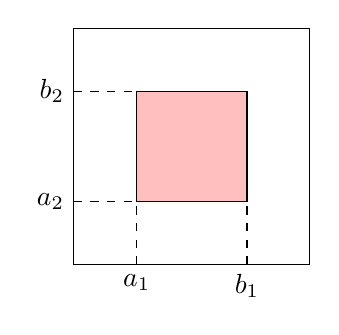
\begin{tikzpicture}
            {
    \def\elemxa{0.8}
    \def\elemxb{2.2}
    \def\elemya{0.8}
    \def\elemyb{2.2}

    \def\minx{0}
    \def\maxx{3}
    \def\miny{0}
    \def\maxy{3}

    \def\firstrect{(\minx,\miny) rectangle (\maxx,\maxy)}
    \def\secondrect{(\elemxa,\elemya) rectangle (\elemxb,\elemyb)}

    \fill[red!25] \secondrect;

    \draw[dashed] (\minx,\elemya) node[left]{$a_2$} -- (\elemxa,\elemya);
    \draw[dashed] (\minx,\elemyb) node[left]{$b_2$} -- (\elemxa,\elemyb);

    \draw[dashed] (\elemxa,\miny) node[below]{$a_1$} -- (\elemxa,\elemya);
    \draw[dashed] (\elemxb,\miny) node[below]{$b_1$} -- (\elemxb,\elemyb);

    \draw[black] \secondrect;
    \draw[black] \firstrect;
}

        \end{tikzpicture}
        \caption{\ref{itm:vert_eigenschaft}. Eigenschaft der Verteilungsfunktion (rote Fläche): ${\mathbb{P}(a_1< X_1\leq b_1,a_2<X_2\leq b_2)}$}
        \label{fig:vert_eigenschaft}
    \end{figure}

    \subsection{Wahrscheinlichkeiten mithilfe der Verteilungsfunktion}\index{Verteilungsfunktion!Wahrscheinlichkeiten|see{Wahrscheinlichkeiten mit Verteilungsfunktion}}\index{Wahrscheinlichkeiten mit Verteilungsfunktion}\label{sec:wahrscheinlichkeiten_verteilungsfunktionen}
    \[\mathbb P(X\le a)=F_X(a),\]
    \[\mathbb P(X<a)=F_X(a-0),\]
    \[\mathbb P(a< X\le b)=F_X(b)-F_X(a),\]
    \[\mathbb P(a< X< b)=F_X(b-0)-F_X(a),\]
    \[\mathbb P(a\le X\le b)=F_X(b)-F_X(a-0),\]
    \[\mathbb P(a\le X< b)=F_X(b-0)-F_X(a-0).\]
    \[\mathbb P( X= a)=F_X(a)-F_X(a-0).\]
    Dabei ist $F(x-0)=\lim\limits_{h\rightarrow 0}F(x-h)$ der linksseitige Grenzwert
    von $F$ in $x$.

    \index{Verteilungsfunktion!{Eigenschaften}|)}


    \section{Unabhängigkeit von Zufallsvariablen}\index{Zufallsvariable!{Unabhängigkeit}|see{Unabhängigkeit von Zufallsvariablen}}\index{Unabhängigkeit von Zufallsvariablen|(}

    \begin{definition}\index{Unabhängigkeit!Verteilung}\label{def:unabhaengigkeit_verteilung}
        Die Zufallsvariablen $(X,Y)$ heißen unabhängig, wenn für
        alle $x_1,\dots x_n$
        \[F_{X_1,\dots,X_n}(x_1,\dots,x_n)=\prod_{i=1}^nF_{X_i}(x_i).\]
        Die unendliche Folge $(X_n,n\in\mathbb N)$ heißt unabhängig, wenn
        jede endliche Teilfolge unabhängig ist.\\


        Wenn die gemeinsame Verteilung diskret bzw. stetig ist, kann man in dieser
        Definition die Verteilungsfunktion durch die Wahrscheinlichkeits- bzw. Dichte-
        funktion ersetzen.
    \end{definition}

    Dafür müssen wir nur die Eigenschaften der Ereignisse auf
    Zufallsvariablen übertragen:

    \begin{definition}
        $X$ und $Y$ heißen unabhängig, wenn $\forall x\in \mathbb R$ und $y\in \mathbb R$
        die Ereignisse $X\le x$ und $Y\le y$ unabhängig sind.

        Das heißt, es muss gelten

        \[
            \mathbb{P}\left(X\le x|Y\le y\right)=\mathbb P(X\le x)
        \]

        oder gleichwertig

        \[
            \mathbb P\left(X\le x\cap Y\le y\right)=
            \mathbb P\left(X\le x\right)\cdot \mathbb P\left(Y\le y\right)
        \]
    \end{definition}

    Mit mehreren Zufallsvariablen muss man wieder zwischen paarweiser und
    totaler Unabhängigkeit unterscheiden. Die $n$ zufälligen Variablen $X_{1},...,X_{n}$
    heißen total unabhängig, wenn für alle $x_{1},...,x_{n}$ gilt:

    \[
    \mathbb P_{X_{1},... ,X_{n}}\left(x_{1},... ,x_{n}\right)=\prod_{i=1}^n{\mathbb P_{i}(x_{i})}
    \]

    \begin{satz}[Faltung von Dichten]\index{Faltung von Dichten}\index{Dichten!Faltung}\label{satz:faltung_dichten} $X$ und $Y$ seien unabhängig mit Dichte $f_X$ und $f_Y$.
        Dann ist die Dichte von $X+Y$ die Faltung von $f_X$ und $f_Y$:
        \[f_{X+Y}(z)=f_X*f_Y(z)=\int_{-\infty}^{\infty} f_X(x)f_Y(z-x)dx.\]
    \end{satz}

    \index{Unabhängigkeit von Zufallsvariablen|)}

    \section{Erwartungswert und Varianz}

    \subsection{Erwartungswert $\mathbb E(X)$ bzw. $\mu_{X}$}\index{Erwartungswert|(}
    \label{sec:erwartungswert}
    Im folgenden Werden die Symbole \gls{symb:mathbbE} und \gls{symb:mu} für den Erwartungswert verwendet.

    \begin{definition}[ von Erwartungswert $\mathbb E$ bzw. $\mu_X$ von $X$]:\\\label{def:erwartungswert}
        Für eine mit Wahrscheinlichkeitsverteilung ${\mathbb P\left(X=x_{j}\right),j=1,2,...,{\infty}}$ verteilte \textbf{diskrete Zufallsvariable} $Y$ gilt:

        \[\mathbb E\left(X\right)=\sum_{j=1}^{{\infty}}{x_{j}\cdot \mathbb P\left(X=x_{j}\right)}\]

        sofern die unendliche Reihe absolut konvergiert. Ansonsten existiert kein Erwartungswert.\\

        Für \textbf{stetige Zufallsvariablen} gilt:
        \[\mathbb E\left(X\right)=\int_{-{\infty}}^{{\infty}}{xf_{X}\left(x\right)}dx\]

        Falls $Y$ \textbf{gemischt verteilt} ist, gilt:
        \[\mathbb E\left(X\right)=\sum_{x}{x\cdot \mathbb P(X=x_{j})}+\int_{-{\infty}}^{{\infty}}{xf_{X}(x)}dx\]
    \end{definition}

    Betrachten wir das anhand unseres Münzspiels (siehe Tabelle \ref{tab:auszahlungen}).\\

    Mit der Wahrscheinlichkeitsverteilung für die Auszahlungen (siehe Abbildung \ref{fig:vert_muenze}):

    \begin{figure}
    \centering
        \begin{tikzpicture}
            {
    \begin{axis}[
        ylabel=Wahrscheinlichkeit,
        xlabel=Auszahlung in Cent,
        axis x line=bottom, % no box around the plot, only x and y axis
        axis y line=left, % the * would suppress the arrow tips
        ymin=0.1,
        ymax=0.6,
        xmin=0.15,
        xmax=100,
        xtick={0,10,30,40,60,80,100},
        enlargelimits=0.15,
        legend pos=north east,
        ybar=-9pt,% configures `bar shift'
        bar width=9pt,
        width=10cm,
        height=5cm,
        clip=false
    ]
    \addplot 
        coordinates {(0,4/8)};

    \addplot 
        coordinates {(20,3/8)};

    \addplot 
        coordinates {(100,1/8)};

    \legend{{0-1x Kopf},{ 2x Kopf },{ 3x Kopf }}

\tikzstyle{vecArrow} = [thick, green, decoration={markings,mark=at position 1 with {\arrow[semithick,green]{open triangle 60}}},
   double distance=1.4pt, shorten >= 5.5pt,
   preaction = {decorate},
   postaction = {draw,line width=1.4pt, white,shorten >= 4.5pt}]

    \node (sp) at (axis cs:20,0.05){};
    \node (down) at (axis cs:20,-0.1){};
    \draw[vecArrow](down)--(sp);

    \end{axis}
}

        \end{tikzpicture}
        \caption{Wahrscheinlichkeitsverteilung für Auszahlung (grüner Pfeil ist Schwerpunkt) siehe Tabelle \ref{tab:auszahlungen}}
        \label{fig:vert_muenze}
    \end{figure}

    Für den Schwerpunkt (grüner Pfeil in Abbildung \ref{fig:vert_muenze}) berechnen wir:

    \[
    \mathbb E\left(X\right)=0\cdot \frac{4}{8}+20\cdot \frac{3}{8}+100\cdot \frac{1}{8}=20
    \]

    \attention {Der Erwartungswert einer Zufallsvariablen ist der Schwerpunkt
    (arithmetisches Mittel) ihrer Verteilung.}

    \subsubsection{Eigenschaften des Erwartungswertes}\index{Erwartungswert!Eigenschaften|see{Eigenschaften des Erwartungswertes}}\index{Eigenschaften des Erwartungswertes}

    \begin{enumerate}[1)]
        \item \textbf{Additivität} Sind $X$, $Y$ zwei Zufallsvariablen, egal ob abhängig oder nicht, mit den
            Erwartungswerten $\mathbb E\left(X\right),\mathbb E\left(Y\right)$, dann gilt:
            \[\mathbb E\left(X+Y\right)=\mathbb E\left(X\right)+\mathbb E(Y)\]
        \item \textbf{Linearität}
            \[\mathbb E\left(aX+b\right)=a\mathbb E\left(X\right)+b\]
        \item \textbf{Monotonie}
            \[X\le Y\Rightarrow \mathbb E\left(X\right)\le \mathbb E(Y)\]
        \item \textbf{Unabhängigkeit}: Wenn $X$ und $Y$ unabhängig sind, dann gilt:
            \[\mathbb E\left(XY\right)=\mathbb E\left(X\right)\mathbb E(Y)\]
    \end{enumerate}

    \begin{satz}\label{satz:unachtsamer_statistiker} \textbf{des unachtsamen Statistikers}\index{Satz des unachtsamen Statistiker}\index{unachtsamer Statistiker!Satz-|see{Satz des unachsamen Statistiker}}
    Siehe Abbildung \ref{fig:unachtsamer_statistiker}.

    $X$ sei stetig verteilt mit der Dichte $f_{X},Y=g\left(X\right)$.
    Um den Erwartungswert von $Y$ zu berechnen, müssen wir nicht die Verteilung von $Y$ berechnen. Wir können
    direkt folgendes Integral verwenden:

    \[\mathbb E\left(Y\right)=\int {g\left(x\right)f_{X}(x)}dx\]

    \end{satz}
    \begin{figure}
    \centering
        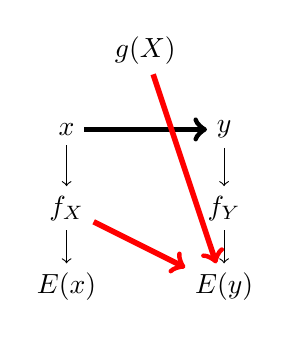
\begin{tikzpicture}
            {
    \def\gxx{0}
    \def\gxy{2}

    \def\xx{-1}
    \def\xy{1}
    \def\yx{1}
    \def\yy{1}

    \def\exx{-1}
    \def\exy{-1}
    \def\eyx{1}
    \def\eyy{-1}

    \def\fxx{-1}
    \def\fxy{0}
    \def\fyx{1}
    \def\fyy{0}

    \node (x) at (\xx,\xy){$x$};
    \node (ex) at (\exx,\exy){$\mathbb E(x)$};
    \node (y) at (\yx,\yy){$y$};
    \node (ey) at (\eyx,\eyy){$\mathbb E(y)$};
    \node (fx) at (\fxx,\fxy){$f_X$};
    \node (fy) at (\fyx,\fyy){$f_Y$};
    \node (gx) at (\gxx,\gxy){$g(X)$};

    \draw[line width=2pt,->](x) -- (y);

    \draw[->](x) -- (fx);
    \draw[->](fx) -- (ex);

    \draw[->](y) -- (fy);
    \draw[->](fy) -- (ey);

    \draw[red,line width=2pt,->](gx) -- (ey);
    \draw[red,line width=2pt,->](fx) -- (ey);
}    
    %\node (sp) at (axis cs:20,0.05){};
    %\node (down) at (axis cs:20,-0.1){};
    %\draw[vecArrow](down)--(sp);

        \end{tikzpicture}
        \caption{Satz des unachtsamen Statistikers (siehe Satz\ref{satz:unachtsamer_statistiker})}
        \label{fig:unachtsamer_statistiker}
    \end{figure}

    \index{Erwartungswert|)}
    \subsection{Varianz}\index{Varianz|(}
    \label{sec:varianz}
    \begin{definition}
    Die Varianz \gls{symb:mathbbV}$(X)$ ist der Mittelwert der quadrierten Abweichungen der
    einzelnen Realisationen vom Schwerpunkt der Verteilung.

    \[\mathbb V\left(X\right)=\mathbb E\left(X-\mathbb E\left(X\right)\right)^{2}=\mathbb E\left(X-\mu\right)^{2}=\sigma ^{2}\]
    \end{definition}

    Für die Berechnung benutzen wir den Erwartungswert (diskret bzw. stetig):

    \[\mathbb V\left(X\right)=\sum_{j=1}^{{\infty}}{\left(x_{j}-\mu\right)^{2}\cdot \mathbb P\left(X=x_{j}\right)}=
    \int_{-{\infty}}^{{\infty}}{\left(x-\mu \right)^{2}f_{X}(x)}dx\]
    \attention{Die Varianz $\mathbb V$ ist ein quadratisches Streuungsmaß}

    \begin{definition}\textbf{Stichprobenvarianz \gls{symb:sn2} mit ML-Schätzer}\index{Stichprobenvarianz!mit ML-Schätzer}
    \index{Varianz!Stichprobe mit ML-Schätzer|see{Stichprobenvarianz!mit ML-Schätzer}}
        \label{def:stichprobenvarianz}%TODO: evtl. noch etwas text
        \[s_n^2= \frac{1}{n} \sum_{i=1}^n\left(x_i-\overline x\right)^2\]
    \end{definition}

    \begin{definition}\textbf{Korrigierte Stichprobenvarianz \gls{symb:sn2}}\index{Stichprobenvarianz!korrigiert|see{Korrigierte Stichprobenvarianz}}\index{Korrigierte Stichprobenvarianz}
        \label{def:korrigierte_stichprobenvarianz}%TODO: evtl. noch etwas text
        \[s_n^2= \frac{1}{n-1} \sum_{i=1}^n\left(x_i-\overline x\right)^2\]
    \end{definition}

    \subsubsection{Verschiebungssatz}
    Wir betrachten die Varianz $\mathbb V\left(X\right)=\mathbb E\left(X-\mathbb E\left(X\right)\right)^{2}$,
    formen um und wenden die Eigenschaften des Erwartungswertes an:

    \[\mathbb V\left(X\right)=\mathbb E\left(X-\mathbb E\left(X\right)\right)^{2}=
        \mathbb E\left(\left(X-\mathbb E\left(X\right)\right)^{2}\right)=
        \mathbb E\left(X^{2}-2X\mathbb E\left(X\right)+\mathbb E\left(X\right)^{2}\right)\]

    Anwendung der Additivität:
    \[\mathbb V\left(X\right)=\mathbb E\left(X^{2}\right)-\mathbb E\left(2X\mathbb E\left(X\right)\right)+\mathbb E\left(\mathbb E\left(X\right)^{2}\right)\]

    Anwendung der Linearität und der Eigenschaft $\mathbb E\left(\mathbb E\left(X\right)\right)=\mathbb E(X)$:
    \[\mathbb V\left(X\right)=\mathbb E\left(X^{2}\right)-2\mathbb E\left(X\mathbb E\left(X\right)\right)+\mathbb E\left(X\right)^{2}=
        \mathbb E\left(X^{2}\right)-2\mathbb E\left(X\right)^{2}+\mathbb E\left(X\right)^{2}\]

    \[\mathbb V\left(X\right)=\mathbb E\left(X^{2}\right)-\mathbb E\left(X\right)^{2}\]

    \begin{satz} Steinerscher Verschiebungssatz\index{Steinerscher Verschiebungssatz}\index{Verschiebungssatz!Steiner-|see{Steinerscher Verschiebungssatz}}
        \label{satz:steinerscher_verschiebungssatz}

    \[
    \mathbb E\left(\left(X-a\right)^{2}\right)=\mathbb V\left(X\right)+\left(\mathbb E\left(X\right)-a\right)^{2}
    \]
    \end{satz}

    \subsubsection{Eigenschaften der Varianz}\index{Varianz!Eigenschaften}
    \begin{definition}[Eigenschaften der Varianz]:\label{def:varianz_eigenschaften}
    \begin{enumerate}[1)]
        \item $\mathbb V\left(X\right)\ge 0$
        \item $\mathbb V\left(X\right)=0$, genau dann, wenn $\mathbb P\left(X=\mathbb E\left(X\right)\right)=1$
        \item $\mathbb V\left(aX+b\right)=a^{2}\mathbb V\left(X\right)$
        \item Wenn $X$ und $Y$ unabhängig sind, dann ist $\mathbb V\left(X+Y\right)=\mathbb V\left(X\right)+\mathbb V(Y)$
    \end{enumerate}
    \end{definition}

    \subsubsection{Kovarianz\index{Kovarianz}}
    \begin{definition}[Kovarianz]:\\
    Die Kovarianz $Cov\left(X,Y\right)$ gibt Aussage darüber, ob hohe Werte
    von $X$ mit hohen Werten von $Y$ oder eher mit niedrigen Werten von $Y$
    einhergehen.

    \begin{itemize}
        \item Die Kovarianz ist positiv, wenn $X$ und $Y$ einen monotonen Zusammenhang
        besitzen, d.h. hohe (niedrige) Werte von $X$ gehen mit hohen (niedrigen)
        Werten von $Y$ einher.
        \item Ist die Kovarianz null, so besteht kein monotoner Zusammenhang zwischen $X$ und $Y$.
    \end{itemize}
    \[Cov\left(X,Y\right)=\mathbb E\left(XY\right)-\mathbb E\left(X\right)\mathbb E\left(Y\right)\]
    \end{definition}
    Damit können wir die Varianz berechnen:
    \[\mathbb V\left(X+Y\right)=\mathbb V\left(X\right)+\mathbb V\left(Y\right)+2Cov\left(X,Y\right)\]
    Wenn die Kovarianz von zwei Zufallsvariablen gleich 0 ist, dann nennen wir sie unkorreliert.

    \subsubsection{Ungleichung von Markov}\index{Ungleichung!von Markov}\index{Markov Ungleichung|see{Ungleichung!von Markov}}
    \begin{definition}[Ungleichung von Markov]:\\
    $X$ sei eine nichtnegative Zufallsvariable und  $\lambda>0$. Dann ist
    \[
    \mathbb P\left(X\ge \lambda \right)\le \frac{1}{\lambda }\mathbb E(X)
    \]
    \end{definition}

    \subsubsection{Ungleichung von Chebychev\index{Ungleichung!von Chebychev}
        \index{Chebychev Ungleichung|see{Ungleichung!von Chebychev}}}

    \begin{definition}[Ungleichung von Chebychev]:\\
        Diese Ungleichung gibt eine allgemeine Schranke an, wie weit eine Zufallsvariable 
        $X$ um ihren Mittelwert streut. Für jede Variable $X$ mit existierender Varianz $\sigma^{2}$ und
        jede beliebige positive Zahl $\lambda$ gilt:

        \[\mathbb P\left(\left|X-\mu \right|\ge \lambda \right)\le \frac{\mathbb V(X)}{\lambda^{2}}\]
        \[\mathbb P\left(\left|X-\mu \right|<\lambda \right)\ge 1-\frac{\mathbb V(X)}{\lambda ^{2}}\]
    \end{definition}

    \begin{bsp}[aus Wikipedia\cite{wiki:002}] Nehmen an, dass Wikipedia-Artikel einen Erwartungswert der Länge von 
    $\mathbb E\left(X\right)=1000$ Zeichen mit einer Standardabweichung von 
    $\sigma_{X}=\sqrt{\mathbb V\left(X\right)}=200$ Zeichen besitzen. 

    Die Wahrscheinlichkeit, dass ein Wikipedia-Artikel eine
    Länge zwischen $600$ und $1400$ $\left(\Rightarrow \lambda=400\right)$ Zeichen hat, berechne sich mit:

    \[
        \mathbb P\left|\left(X-1000\right|<400\right)=1-\frac{200^{2}}{400^{2}}=1-\frac{1}{4}=75
    \]
    \end{bsp}

    \subsubsection{Ungleichung von Kolmogorov\index{Ungleichung!von Kolmogorov}
        \index{Kolmogorov Ungleichung|see{Ungleichung!von Kolmogorov}}}
    \begin{definition}\textbf{Kolmogorov-Ungleichung}
    Die Kolmogorov-Ungleichung ist eine sogenannte Maximal-Ungleichung aus
    der Stochastik. Seien $X_{1},... ,X_{n}$ unabhängige Zufallsvariablen mit
    Erwartungswert 0, und zusätzlich $S_{0}=0,$ und $S_{n}=X_{1}+... +X_{n}$. Dann ist

    \[\mathbb P\left(\max_{k\le n}\left(S_{k}\right)\ge \lambda\right)\le 
        \frac{\mathbb V\left(S_{n}\right)}{\lambda ^{2}}\]
    \end{definition}
    
    \index{Varianz|)}


    \section{Folgen von Zufallsvariablen}\index{Zufallsvariable!Folgen|see{Folgen von Zufallsvariablen}}\index{Folgen von Zufallsvariablen|(}

    Nun untersuchen wir Folgen von Zufallsvariablen $X_{1},...,X_{n},$ die unabhängig und identisch
    verteilt sind, abgekürzt \gls{symb:iid} (independent and identically distributed). 
    Einfachstes Beispiel sind drei unabhängige Münzwürfe.

    \subsection{Schwaches Gesetz der großen Zahlen\index{Gesetz!Schwaches G. der gr. Z.|see{Schwaches G. der gr. Z.}}\index{Schwaches G. der gr. Z.|(}}

    Bei geringem Stichprobenumfang n ist die Chebychev-Ungleichung sehr
    ungenau, sie wird aber genauer, je größer n wird. Wir gehen von n
    Zufallsvariablen aus und bilden uns den Mittelwert:

    \[\overline{X}^{\left(n\right)}=\frac{1}{n}\sum_{i=1}^{n}X_{i}\]

    Der Erwartungswert von i.i.d Zufallsvariablen ist immer gleich, somit gilt:

    \[\mathbb E\left(\overline{X}^{\left(n\right)}\right)=\mu\]

    Da die Varianz ein quadratisches Streuungsmaß ist, folgt:

    \[\mathbb V\left(\overline{X}^{\left(n\right)}\right)=
        \mathbb V\left(\frac{1}{n}\sum_{i=1}^{n}X_{i}\right)=
        \frac{1}{n^{2}}\mathbb V\left(\sum_{i=1}^{n}X_{i}\right)\]

    denn beim Ausklammern der Konstante $\frac{1}{n}$ wird diese quadriert.

    \[\frac{1}{n^{2}}\mathbb V\left(\sum_{i=1}^{n}X_{i}\right)=\frac{1}{n^{2}}n\sigma ^{2}=\frac{\sigma^{2}}{n}\]

    \attention {Die letzte Umformung kommt aus der Summenregel für unkorrelierte
    Zufallsvariablen: $\mathbb V\left(\sum _{i=1}^{n}X_{i}\right)=\sum _{i=1}^{n}{\mathbb V(X_{i})}$}

    Nun benutzen wir die Ungleichung von Chebychev und passen sie an:

    \[\mathbb P\left(\left|{\overline{X}}^{\left(n\right)}-\mu
    \right|<\lambda \right)\ge 1-\frac{\frac{\sigma ^{2}}{n}}{\lambda
    ^{2}}\]
    \[\mathbb P\left(\left|{\overline{X}}^{\left(n\right)}-\mu \right|<\lambda
    \right)\ge 1-\frac{\sigma ^{2}}{n\lambda ^{2}}\]

    Schlussendlich schicken wir n gegen unendlich und beachten, dass die
    Wahrscheinlichkeit nie größer als Eins werden kann:

    \[\lim_{n\rightarrow{\infty}}\mathbb P\left(\left|{\overline{X}}^{\left(n\right)}-\mu
    \right|<\lambda \right)\ge 1\]
    \begin{definition}\textbf{Schwaches Gesetz der großen Zahlen}\\
        Es sei $\left(X_{n}\right)_{n\in N}$ eine Folge von i.i.d.-zufälligen Variablen mit 
        $\mathbb E\left(X_{n}\right)=\mu$. Dann gilt $\forall\epsilon >0$:

    \[\lim_{n\rightarrow\infty}\mathbb P\left(\left|{\overline{X}}^{\left(n\right)}-\mu
    \right|<\epsilon \right)=1\]
    \end{definition}

    Das schwache Gesetz der großen Zahlen sagt uns also, dass mit
    steigender Anzahl von Zufallsvariablen große Abweichungen immer
    unwahrscheinlicher werden.

    \index{Schwaches G. der gr. Z.|)}

    \subsection{Starkes Gesetz der großen Zahlen\index{Gesetz!Starkes G. der gr. Z.|see{Starkes G. der gr. Z.}}\index{Starkes G. der gr. Z.|(}}\label{sec:starkes_gesetz_grossen_zahlen}

    Das starke Gesetz der großen Zahlen bedeutet, dass
    \[\lim_{n\rightarrow\infty}{\overline{X}}^{\left(n\right)}=\mu\]
    nicht immer, aber {\quotedblbase}so gut wie immer{\textquotedblleft}
    gilt.

    \begin{definition}
    Es sei $\left(X_{n}\right)_{n\in \mathbb N}$ eine
    Folge von i.i.d.-zufälligen Variablen mit
    ${\mathbb E\left(X_{i}\right)=\mu}$
    Dann gilt:

    \[\mathbb P\left(\underset{n\rightarrow
    {\infty}}{{lim}}{\overline{X}}^{\left(n\right)}=\mu \right)=1\]

    Man sagt: ${\overline{X}}^{\left(n\right)}$ konvergiert fast sicher gegen $\mu$.
    \end{definition}
    \index{Starkes G. der gr. Z.|)}

    \subsection{Zentraler Grenzwertsatz\index{Grenzwertsatz!Zentraler-|see{Zentraler Grenzwertsatz}}\index{Zentraler Grenzwertsatz|(}}

    Dafür führen wir zuerst den Begriff der standardisieren Zufallsvariable ein.

    \begin{definition}\textbf{Standardisierte Zufallsvariable}\index{Standardisierte Zufallsvariable}\index{Zufallsvariable!standardisierte}\\
    Eine Zufallsvariable $X$ mit Erwartungswert gleich null und Varianz gleich
    eins heißt standardisierte Zufallsvariable. Ist $X$ eine beliebige
    Zufallsvariable mit $\mathbb E\left(X\right)=\mu$ und $\mathbb V\left(X\right)=\sigma^{2}$,
    dann heißt 
    \[X^*=\frac{X-\mu }{\sigma }\]
    $\sigma$ bezeichnet dabei die Standardabweichung $\sigma=\sqrt{\mathbb V\left(X\right)}$

    die Standardisierte von $X$. Der Vorgang selbst heißt Standardisierung. Für die standardisierte Variable $X^*$ gilt:

    \[\mathbb E\left(X^*\right)=0\]
    \[\mathbb V\left(X^*\right)=1\]
    \end{definition}

    Beim zentralen Grenzwertsatz berechnen wir zuerst die Summe von $n$ i.i.d. Zufallsvariablen mit 
    $\mathbb E\left(X\right)=\mu $ und $\mathbb V\left(X\right)=\sigma^{2}$:

    \[S_{n}=X_{1}+\ldots +X_{n}\]
    \[\mathbb E\left(S_{n}\right)=n\mu\]
    \[\mathbb V\left(S_{n}\right)=n\sigma^{2}\]

    Wir standardisieren $S_{n}$:
    \[S_{n}^*=\frac{S_{n}-n\mu}{\sqrt{n\sigma^{2}}}\]

    \begin{satz}\textbf{Zentraler Grenzwertsatz:}\label{satz:zentraler_grenzwertsatz}\\
    Der zentrale Grenzwertsatz besagt, dass die Verteilungsfunktion 
    $S_{n}^*$ für $n\rightarrow\infty$
    punktweise gegen die Verteilungsfunktion der Standardnormalverteilung $\mathcal N\left(0,1\right)$ konvergiert. 
    Ist $\Phi\left(z\right)$ die Verteilungsfunktion von $\mathcal N\left(0,1\right)$, 
    dann bedeutet dies, dass für jedes reelle $z$ gilt:

    \[\lim_{n\rightarrow\infty}\mathbb P\left(S_{n}^*\le z\right)=
    \lim_{n\rightarrow\infty}\mathbb P\left(\frac{S_{n}-n\mu}{\sqrt{n\sigma^{2}}}\le z\right)=
    \Phi \left(z\right)=\int_{-\infty}^{z}{\frac{1}{\sqrt{2\pi}}e^{\frac{-x^{2}}{2}}}dx\]
    \end{satz}

    \index{Zentraler Grenzwertsatz|)}
    \index{Folgen von Zufallsvariablen|)}

    \section{Diskrete Verteilungen}\index{Verteilung!Diskret|see{Diskrete Verteilung}}\index{Diskrete Verteilung|(}\label{sec:diskrete_verteilungen}

    \subsection{Binomialverteilung\index{Binomialverteilung}\index{Verteilung!Binomial-|see{Binomialverteilung}}}\label{sec:binomialverteilung}
    \label{sec:binomialverteilung}
    {
        \begin{figure}
            \def\nval{30}
            \subfigure[Wahrscheinlichkeitsfunktion mit $n=\nval$]{
                \begin{tikzpicture}
                    {
    \def\pvala{0.5}
    \def\pvalb{0.25}
    \def\pvalc{0.75}
    \def\pvald{0.9}

    \pgfmathtruncatemacro{\maxval}{\nval}

    \begin{axis}[
        domain=-4:4,
        axis x line=bottom, % no box around the plot, only x and y axis
        axis y line=left, % the * would suppress the arrow tips
        legend style={at={(0.67\nval,1.2)}},
        xlabel={k},
        ylabel={p},%TODO: was ist diese Achse?
        samples=200,
        height=5cm,
        width=7cm,
        clip=false]

        \pgfkeys{/pgf/fpu=true}
        \pgfkeys{/pgf/number format/.cd,fixed,precision=5}

        \def\x{1}
        \pgfmathparse{binomial_distribution(\nval,\x,\pvalb)}
        \addplot[continuityblue] coordinates{(\x,\pgfmathresult)};
        \addlegendentry[align=left]{\scriptsize{$\mathcal B(k|\nval,\pvalb)$}};

        \pgfmathparse{binomial_distribution(\nval,\x,\pvalc)}
        \addplot[continuitygreen] coordinates{(\x,\pgfmathresult)};
        \addlegendentry[align=left]{\scriptsize{$\mathcal B(k|\nval,\pvalc)$}};

        \pgfmathparse{binomial_distribution(\nval,\x,\pvald)}
        \addplot[continuityorange] coordinates{(\x,\pgfmathresult)};
        \addlegendentry[align=left]{\scriptsize{$\mathcal B(k|\nval,\pvald)$}};

        \pgfmathparse{binomial_distribution(\nval,\x,\pvala)}
        \addplot[continuityred] coordinates{(\x,\pgfmathresult)};
        \addlegendentry[align=left]{\scriptsize{$\mathcal B(k|\nval,\pvala)$}};

        \foreach \x in {2,...,\maxval} {
            \pgfkeys{/pgf/fpu=false}
            \pgfmathtruncatemacro{\nextx}{\x+1}
            \pgfkeys{/pgf/fpu=true}
            \pgfkeys{/pgf/number format/.cd,fixed,precision=5}

            \pgfmathparse{binomial_distribution(\nval,\x,\pvalb)}
            \addplot[continuityblue,forget plot] coordinates{(\x,\pgfmathresult)};

            \pgfmathparse{binomial_distribution(\nval,\x,\pvalc)}
            \addplot[continuitygreen,forget plot] coordinates{(\x,\pgfmathresult)};

            \pgfmathparse{binomial_distribution(\nval,\x,\pvald)}
            \addplot[continuityorange,forget plot] coordinates{(\x,\pgfmathresult)};

            \pgfmathparse{binomial_distribution(\nval,\x,\pvala)}
            \addplot[continuityred,forget plot] coordinates{(\x,\pgfmathresult)};
        }
        \pgfkeys{/pgf/fpu=false}


    \end{axis}
}
            
                \end{tikzpicture}
                \label{fig:binomial_dist_a}
            }
            \def\nval{15}
            \subfigure[Wahrscheinlichkeitsfunktion mit $n=\nval$]{
                \begin{tikzpicture}
                    {
    \def\pvala{0.5}
    \def\pvalb{0.25}
    \def\pvalc{0.75}
    \def\pvald{0.9}

    \pgfmathtruncatemacro{\maxval}{\nval}

    \begin{axis}[
        domain=-4:4,
        axis x line=bottom, % no box around the plot, only x and y axis
        axis y line=left, % the * would suppress the arrow tips
        legend style={at={(0.67\nval,1.2)}},
        xlabel={k},
        ylabel={p},%TODO: was ist diese Achse?
        samples=200,
        height=5cm,
        width=7cm,
        clip=false]

        \pgfkeys{/pgf/fpu=true}
        \pgfkeys{/pgf/number format/.cd,fixed,precision=5}

        \def\x{1}
        \pgfmathparse{binomial_distribution(\nval,\x,\pvalb)}
        \addplot[continuityblue] coordinates{(\x,\pgfmathresult)};
        \addlegendentry[align=left]{\scriptsize{$\mathcal B(k|\nval,\pvalb)$}};

        \pgfmathparse{binomial_distribution(\nval,\x,\pvalc)}
        \addplot[continuitygreen] coordinates{(\x,\pgfmathresult)};
        \addlegendentry[align=left]{\scriptsize{$\mathcal B(k|\nval,\pvalc)$}};

        \pgfmathparse{binomial_distribution(\nval,\x,\pvald)}
        \addplot[continuityorange] coordinates{(\x,\pgfmathresult)};
        \addlegendentry[align=left]{\scriptsize{$\mathcal B(k|\nval,\pvald)$}};

        \pgfmathparse{binomial_distribution(\nval,\x,\pvala)}
        \addplot[continuityred] coordinates{(\x,\pgfmathresult)};
        \addlegendentry[align=left]{\scriptsize{$\mathcal B(k|\nval,\pvala)$}};

        \foreach \x in {2,...,\maxval} {
            \pgfkeys{/pgf/fpu=false}
            \pgfmathtruncatemacro{\nextx}{\x+1}
            \pgfkeys{/pgf/fpu=true}
            \pgfkeys{/pgf/number format/.cd,fixed,precision=5}

            \pgfmathparse{binomial_distribution(\nval,\x,\pvalb)}
            \addplot[continuityblue,forget plot] coordinates{(\x,\pgfmathresult)};

            \pgfmathparse{binomial_distribution(\nval,\x,\pvalc)}
            \addplot[continuitygreen,forget plot] coordinates{(\x,\pgfmathresult)};

            \pgfmathparse{binomial_distribution(\nval,\x,\pvald)}
            \addplot[continuityorange,forget plot] coordinates{(\x,\pgfmathresult)};

            \pgfmathparse{binomial_distribution(\nval,\x,\pvala)}
            \addplot[continuityred,forget plot] coordinates{(\x,\pgfmathresult)};
        }
        \pgfkeys{/pgf/fpu=false}


    \end{axis}
}
            
                \end{tikzpicture}
                \label{fig:binomial_dist_b}
            }

            \def\nval{30}
            \subfigure[Binomialverteilung mit $n=\nval$]{
                \begin{tikzpicture}
                    {
    \def\pvala{0.5}
    \def\pvalb{0.25}
    \def\pvalc{0.75}
    \def\pvald{0.9}

    \pgfmathtruncatemacro{\maxval}{\nval}

    \begin{axis}[
        domain=-4:4,
        axis x line=bottom, % no box around the plot, only x and y axis
        axis y line=left, % the * would suppress the arrow tips
        legend pos=north west,
        xlabel={k},
        ylabel={p},%TODO: was ist diese Achse?
        samples=200,
        height=5cm,
        width=7cm,
        clip=false]

        \pgfkeys{/pgf/fpu=true}
        \pgfkeys{/pgf/number format/.cd,fixed,precision=5}

        \def\x{1}
        \def\nextx{2}
        %\foreach \x/\y [remember=\x as \lastx (initially A)] in {B/2,C/3,D/4,E/5}
        \pgfmathparse{binomial_distribution(\nval,\x,\pvalb)}
        \xdef\tvalb{\pgfmathresult}
        \addplot[blue,forget plot] coordinates{(\x,\tvalb)(\nextx,\tvalb)};
        \addplot[continuityblue] coordinates{(\x,\tvalb)};
        \addlegendentry[align=left]{\scriptsize{$\mathcal B(k|\nval,\pvalb)$}};

        \pgfmathparse{binomial_distribution(\nval,\x,\pvalc)}
        \xdef\tvalc{\pgfmathresult}
        \addplot[green,forget plot] coordinates{(\x,\tvalc)(\nextx,\tvalc)};
        \addplot[continuitygreen] coordinates{(\x,\tvalc)};
        \addlegendentry[align=left]{\scriptsize{$\mathcal B(k|\nval,\pvalc)$}};

        \pgfmathparse{binomial_distribution(\nval,\x,\pvald)}
        \xdef\tvald{\pgfmathresult}
        \addplot[orange,forget plot] coordinates{(\x,\tvald)(\nextx,\tvald)};
        \addplot[continuityorange] coordinates{(\x,\tvald)};
        \addlegendentry[align=left]{\scriptsize{$\mathcal B(k|\nval,\pvald)$}};

        \pgfmathparse{binomial_distribution(\nval,\x,\pvala)}
        \xdef\tvala{\pgfmathresult}
        \addplot[red,forget plot] coordinates{(\x,\tvala)(\nextx,\tvala)};
        \addplot[continuityred] coordinates{(\x,\tvala)};
        \addlegendentry[align=left]{\scriptsize{$\mathcal B(k|\nval,\pvala)$}};

        \foreach \x [remember=\x as \lastx (initially 0)] in {2,...,\maxval} {
            \pgfkeys{/pgf/fpu=false}
            \pgfmathtruncatemacro{\nextx}{\x+1}
            \pgfkeys{/pgf/fpu=true}
            \pgfkeys{/pgf/number format/.cd,fixed,precision=5}

            \pgfmathparse{\tvalb+binomial_distribution(\nval,\x,\pvalb)}
            \xdef\tvalb{\pgfmathresult}
            \addplot[blue,forget plot] coordinates{(\x,\tvalb)(\nextx,\tvalb)};
            \addplot[continuityblue,forget plot] coordinates{(\x,\tvalb)};

            \pgfmathparse{\tvalc+binomial_distribution(\nval,\x,\pvalc)}
            \xdef\tvalc{\pgfmathresult}
            \addplot[green,forget plot] coordinates{(\x,\tvalc)(\nextx,\tvalc)};
            \addplot[continuitygreen,forget plot] coordinates{(\x,\tvalc)};

            \pgfmathparse{\tvald+binomial_distribution(\nval,\x,\pvald)}
            \xdef\tvald{\pgfmathresult}
            \addplot[orange,forget plot] coordinates{(\x,\tvald)(\nextx,\tvald)};
            \addplot[continuityorange,forget plot] coordinates{(\x,\tvald)};

            \pgfmathparse{\tvala+binomial_distribution(\nval,\x,\pvala)}
            \xdef\tvala{\pgfmathresult}
            \addplot[red,forget plot] coordinates{(\x,\tvala)(\nextx,\tvala)};
            \addplot[continuityred,forget plot] coordinates{(\x,\tvala)};
        }
        \pgfkeys{/pgf/fpu=false}


    \end{axis}
}
            
                \end{tikzpicture}
                \label{fig:binomial_dist_c}
            }
            \def\nval{15}
            \subfigure[Binomialverteilung mit $n=\nval$]{
                \begin{tikzpicture}
                    {
    \def\pvala{0.5}
    \def\pvalb{0.25}
    \def\pvalc{0.75}
    \def\pvald{0.9}

    \pgfmathtruncatemacro{\maxval}{\nval}

    \begin{axis}[
        domain=-4:4,
        axis x line=bottom, % no box around the plot, only x and y axis
        axis y line=left, % the * would suppress the arrow tips
        legend pos=north west,
        xlabel={k},
        ylabel={p},%TODO: was ist diese Achse?
        samples=200,
        height=5cm,
        width=7cm,
        clip=false]

        \pgfkeys{/pgf/fpu=true}
        \pgfkeys{/pgf/number format/.cd,fixed,precision=5}

        \def\x{1}
        \def\nextx{2}
        %\foreach \x/\y [remember=\x as \lastx (initially A)] in {B/2,C/3,D/4,E/5}
        \pgfmathparse{binomial_distribution(\nval,\x,\pvalb)}
        \xdef\tvalb{\pgfmathresult}
        \addplot[blue,forget plot] coordinates{(\x,\tvalb)(\nextx,\tvalb)};
        \addplot[continuityblue] coordinates{(\x,\tvalb)};
        \addlegendentry[align=left]{\scriptsize{$\mathcal B(k|\nval,\pvalb)$}};

        \pgfmathparse{binomial_distribution(\nval,\x,\pvalc)}
        \xdef\tvalc{\pgfmathresult}
        \addplot[green,forget plot] coordinates{(\x,\tvalc)(\nextx,\tvalc)};
        \addplot[continuitygreen] coordinates{(\x,\tvalc)};
        \addlegendentry[align=left]{\scriptsize{$\mathcal B(k|\nval,\pvalc)$}};

        \pgfmathparse{binomial_distribution(\nval,\x,\pvald)}
        \xdef\tvald{\pgfmathresult}
        \addplot[orange,forget plot] coordinates{(\x,\tvald)(\nextx,\tvald)};
        \addplot[continuityorange] coordinates{(\x,\tvald)};
        \addlegendentry[align=left]{\scriptsize{$\mathcal B(k|\nval,\pvald)$}};

        \pgfmathparse{binomial_distribution(\nval,\x,\pvala)}
        \xdef\tvala{\pgfmathresult}
        \addplot[red,forget plot] coordinates{(\x,\tvala)(\nextx,\tvala)};
        \addplot[continuityred] coordinates{(\x,\tvala)};
        \addlegendentry[align=left]{\scriptsize{$\mathcal B(k|\nval,\pvala)$}};

        \foreach \x [remember=\x as \lastx (initially 0)] in {2,...,\maxval} {
            \pgfkeys{/pgf/fpu=false}
            \pgfmathtruncatemacro{\nextx}{\x+1}
            \pgfkeys{/pgf/fpu=true}
            \pgfkeys{/pgf/number format/.cd,fixed,precision=5}

            \pgfmathparse{\tvalb+binomial_distribution(\nval,\x,\pvalb)}
            \xdef\tvalb{\pgfmathresult}
            \addplot[blue,forget plot] coordinates{(\x,\tvalb)(\nextx,\tvalb)};
            \addplot[continuityblue,forget plot] coordinates{(\x,\tvalb)};

            \pgfmathparse{\tvalc+binomial_distribution(\nval,\x,\pvalc)}
            \xdef\tvalc{\pgfmathresult}
            \addplot[green,forget plot] coordinates{(\x,\tvalc)(\nextx,\tvalc)};
            \addplot[continuitygreen,forget plot] coordinates{(\x,\tvalc)};

            \pgfmathparse{\tvald+binomial_distribution(\nval,\x,\pvald)}
            \xdef\tvald{\pgfmathresult}
            \addplot[orange,forget plot] coordinates{(\x,\tvald)(\nextx,\tvald)};
            \addplot[continuityorange,forget plot] coordinates{(\x,\tvald)};

            \pgfmathparse{\tvala+binomial_distribution(\nval,\x,\pvala)}
            \xdef\tvala{\pgfmathresult}
            \addplot[red,forget plot] coordinates{(\x,\tvala)(\nextx,\tvala)};
            \addplot[continuityred,forget plot] coordinates{(\x,\tvala)};
        }
        \pgfkeys{/pgf/fpu=false}


    \end{axis}
}
            
                \end{tikzpicture}
                \label{fig:binomial_dist_d}
            }
            \caption{Die Binomialverteilung}
            \label{fig:binomial_dist}
        \end{figure}
    }

    \begin{bsp}\textbf{Münzwurf:}\\ 
    Bezeichnen wir die Wahrscheinlichkeit von \textbf{Kopf mit} $p$, so ergibt sich die Wahrscheinlichkeit von 
    \textbf{Zahl} mit $1-p$.

    Ist $X$ die Anzahl der Kopfwürfe bei $n$ Würfen, so tritt das Ereignis $X=k$ genau dann auf, wenn in einer
    Wurfsequenz $(... K ... Z ... Z ...)$ genau $k$-mal $K$ auftritt und daher auch $(n-k)$ mal $Z$. 
    Die Wahrscheinlichkeit einer solchen Sequenz ist 
    \[p^{k}\left(1-p\right)^{n-k}\]
    Dabei kann die Reihenfolge egal sein. Wir müssen also noch wissen, wie viele Möglichkeiten es gibt, 
    aus $n$ Würfen, $k$ auszuwählen:

    \[\binom{n}{k}\]
    \end{bsp}

    Sie beschreibt die Anzahl der Erfolge in einer Serie von gleichartigen und unabhängigen Versuchen, die jeweils genau zwei mögliche Ergebnisse haben („Erfolg“ oder „Misserfolg“). (Wikipedia \cite{wiki:003})

    Damit haben wir die Binomialverteilung (siehe Abbildung \ref{fig:binomial_dist}) definiert:
    \begin{definition}\textbf{Binomialverteilung}
    \[
    \mathcal B\left(k|n,p\right)=
    \binom{n}{k}p^{k}\left(1-p\right)^{n-k}k=0,1,...,n
    \]
    \[\mathbb E\left(X\right)=np\]
    \[\mathbb V\left(X\right)=np(1-p)\]
    \end{definition}

    Für die Binomialverteilung existiert ein \textbf{Additionstheorem}:

    \[\text{Aus}
        \begin{cases}X\sim\mathcal B_n(\theta)\\Y\sim\mathcal B_n(\theta)\end{cases} 
        \text{folgt}X+Y\sim\mathcal B_{n+m}(\theta)\]

    Existieren nicht nur zwei Möglichkeiten, kann die Binomialverteilung mit der Polynomialverteilung
    vertauscht werden. Es sind $r,w,... ,g$ die Anzahl der einzelnen Elemente (z.B. rote, weiße und grüne) und 
    $\theta_{r},\theta_{w},...,\theta_{g}$ die entsprechenden Wahrscheinlichkeiten:

    \[
    \mathbb P\left(r,w,\ldots ,g\right)=
        \frac{n!}{r!w!\ldots g!}\left(\theta_{r}\right)^{r}\left(\theta_{w}\right)^{w}\ldots \left(\theta_{g}\right)^{g}
    \]

    \subsection{Gleichverteilung\index{Gleichverteilung!diskret}\index{Verteilung!Gleich-(diskret)|see{Gleichverteilung!diskret}}}\label{sec:gleichverteilung_diskret}

    {
        \begin{figure}
            \def\bval{10}
            \def\aval{2}
            \subfigure[Wahrscheinlichkeitsfunktion]{
                \begin{tikzpicture}
                    {
    \begin{axis}[
        domain=-4:4,
        axis x line=bottom, % no box around the plot, only x and y axis
        axis y line=left, % the * would suppress the arrow tips
        legend pos=north west,
        xlabel={k},
        ylabel={p},%TODO: was ist diese Achse?
        samples=200,
        height=5cm,
        width=7cm,
        clip=false]

        \pgfkeys{/pgf/fpu=true}
        \pgfkeys{/pgf/number format/.cd,fixed,precision=5}

        \def\x{1}
        \addplot[continuityblue] coordinates{(\x,0)};
        \addlegendentry[align=left]{\scriptsize{$\mathcal D(\aval,\bval)$}};

        \foreach \x in {\aval,...,\bval} {
            \pgfkeys{/pgf/fpu=false}
            \pgfmathtruncatemacro{\nextx}{\x+1}
            \pgfkeys{/pgf/fpu=true}
            \pgfkeys{/pgf/number format/.cd,fixed,precision=5}

            \pgfmathparse{1/(\bval-\aval+1)}
            \addplot[continuityblue,forget plot] coordinates{(\x,\pgfmathresult)};
        }

        \pgfkeys{/pgf/fpu=false}

        \pgfmathtruncatemacro{\x}{\bval+1}
        \addplot[continuityblue] coordinates{(\x,0)};
    \end{axis}
}
            
                \end{tikzpicture}
                \label{fig:gleich_dist_a}
            }
            \subfigure[Gleichverteilung]{
                \begin{tikzpicture}
                    {
    \begin{axis}[
        domain=-4:4,
        axis x line=bottom, % no box around the plot, only x and y axis
        axis y line=left, % the * would suppress the arrow tips
        legend pos=north west,
        xlabel={k},
        ylabel={p},%TODO: was ist diese Achse?
        samples=200,
        height=5cm,
        width=7cm,
        clip=false]

        \pgfkeys{/pgf/fpu=true}
        \pgfkeys{/pgf/number format/.cd,fixed,precision=5}

        \def\x{1}
        \def\nextx{2}
        \addplot[continuityblue] coordinates{(\x,0)};
        \xdef\tval{0}
        \addplot[blue,forget plot] coordinates{(\x,\tval)(\nextx,\tval)};
        \addplot[continuityblue] coordinates{(\x,\tval)};
        \addlegendentry[align=left]{\scriptsize{$\mathcal D(\aval,\bval)$}};

        \foreach \x [remember=\x as \lastx (initially 0)] in {\aval,...,\bval} {
            \pgfkeys{/pgf/fpu=false}
            \pgfmathtruncatemacro{\nextx}{\x+1}
            \pgfkeys{/pgf/fpu=true}
            \pgfkeys{/pgf/number format/.cd,fixed,precision=5}

            \pgfmathparse{\tval+1/(\bval-\aval+1)}
            \xdef\tval{\pgfmathresult}
            \addplot[blue,forget plot] coordinates{(\x,\tval)(\nextx,\tval)};
            \addplot[continuityblue,forget plot] coordinates{(\x,\tval)};

        }
        \pgfkeys{/pgf/fpu=false}


    \end{axis}
}
            
                \end{tikzpicture}
                \label{fig:gleich_dist_b}
            }
            \caption{Die Gleichverteilung}
            \label{fig:gleich_dist}
        \end{figure}
    }

    \begin{bsp}
    Die Gleichverteilung beschreibt den Wurf eines idealen $n$-Seiten Würfels. (siehe Abbildung \ref{fig:gleich_dist})
    \end{bsp}

    \begin{definition}
    \[\mathbb P\left(X=k\right)=\frac{1}{n}\]
    \[\mathbb E\left(X\right)=\frac{n+1}{2}\]
    \[\mathbb V\left(X\right)=\frac{n^{2}-1}{12}\]
    \end{definition}
    
    Befindet sich $k$ in einem beliebigen Intervall $a\leq k\le b$, so gilt analog:

    \[\mathbb P\left(X=k\right)=\frac{1}{b-a+1}\]
    \[\mathbb E\left(X\right)=\frac{b+a}{2}\]
    \[\mathbb V\left(X\right)=\frac{\left(b-a\right)^{2}-1}{12}\]
    
    \subsection{Geometrische Verteilung\index{Geometrische Verteilung}\index{Verteilung!Geometrische-|see{Geometrische Verteilung}}}
    \label{sec:geometrische_verteilung}
    {
        \begin{figure}
            \def\nval{10}
            \def\pvala{0.8}
            \def\pvalb{0.5}
            \def\pvalc{0.2}
            \subfigure[Wahrscheinlichkeitsfunktion]{
                \begin{tikzpicture}
                    {
    \begin{axis}[
        domain=-4:4,
        axis x line=bottom, % no box around the plot, only x and y axis
        axis y line=left, % the * would suppress the arrow tips
        legend pos=north east,
        ymin=0,
        ymax=1,
        xlabel={k},
        ylabel={p},%TODO: was ist diese Achse?
        samples=200,
        height=5cm,
        width=7cm,
        clip=false]

        \pgfkeys{/pgf/fpu=true}
        \pgfkeys{/pgf/number format/.cd,fixed,precision=5}

        \def\x{1}
        \pgfmathparse{\pvala*(1-\pvala)^(\x-1)}
        \addplot[continuityblue] coordinates{(\x,\pgfmathresult)};
        \addlegendentry[align=left]{\scriptsize{$\mathcal G(\pvala)$}};

        \pgfmathparse{\pvalb*(1-\pvalb)^(\x-1)}
        \addplot[continuityred] coordinates{(\x,\pgfmathresult)};
        \addlegendentry[align=left]{\scriptsize{$\mathcal G(\pvalb)$}};

        \pgfmathparse{\pvalc*(1-\pvalc)^(\x-1)}
        \addplot[continuitygreen] coordinates{(\x,\pgfmathresult)};
        \addlegendentry[align=left]{\scriptsize{$\mathcal G(\pvalc)$}};

        \foreach \x in {2,...,\nval} {
            \pgfkeys{/pgf/fpu=false}
            \pgfmathtruncatemacro{\nextx}{\x+1}
            \pgfkeys{/pgf/fpu=true}
            \pgfkeys{/pgf/number format/.cd,fixed,precision=5}

            \pgfmathparse{\pvala*(1-\pvala)^(\x-1)}
            \addplot[continuityblue,forget plot] coordinates{(\x,\pgfmathresult)};

            \pgfmathparse{\pvalb*(1-\pvalb)^(\x-1)}
            \addplot[continuityred,forget plot] coordinates{(\x,\pgfmathresult)};

            \pgfmathparse{\pvalc*(1-\pvalc)^(\x-1)}
            \addplot[continuitygreen,forget plot] coordinates{(\x,\pgfmathresult)};
        }

        \pgfkeys{/pgf/fpu=false}
    \end{axis}
}
            
                \end{tikzpicture}
                \label{fig:geomet_dist_a}
            }
            \subfigure[Geometrische Verteilung]{
                \begin{tikzpicture}
                    {
    \begin{axis}[
        domain=-4:4,
        axis x line=bottom, % no box around the plot, only x and y axis
        axis y line=left, % the * would suppress the arrow tips
        legend pos=south east,
        ymin=0,
        ymax=1,
        xlabel={k},
        ylabel={p},%TODO: was ist diese Achse?
        samples=200,
        height=5cm,
        width=7cm,
        clip=false]

        \pgfkeys{/pgf/fpu=true}
        \pgfkeys{/pgf/number format/.cd,fixed,precision=5}

        \def\x{1}
        \def\nextx{2}
        \pgfmathparse{\pvala*(1-\pvala)^(\x-1)}
        \xdef\tvala{\pgfmathresult}
        \addplot[blue,forget plot] coordinates{(\x,\tvala)(\nextx,\tvala)};
        \addplot[continuityblue] coordinates{(\x,\pgfmathresult)};
        \addlegendentry[align=left]{\scriptsize{$\mathcal G(\pvala)$}};

        \pgfmathparse{\pvalb*(1-\pvalb)^(\x-1)}
        \xdef\tvalb{\pgfmathresult}
        \addplot[red,forget plot] coordinates{(\x,\tvalb)(\nextx,\tvalb)};
        \addplot[continuityred] coordinates{(\x,\pgfmathresult)};
        \addlegendentry[align=left]{\scriptsize{$\mathcal G(\pvalb)$}};

        \pgfmathparse{\pvalc*(1-\pvalc)^(\x-1)}
        \xdef\tvalc{\pgfmathresult}
        \addplot[green,forget plot] coordinates{(\x,\tvalc)(\nextx,\tvalc)};
        \addplot[continuitygreen] coordinates{(\x,\pgfmathresult)};
        \addlegendentry[align=left]{\scriptsize{$\mathcal G(\pvalc)$}};

        \foreach \x in {2,...,\nval} {
            \pgfkeys{/pgf/fpu=false}
            \pgfmathtruncatemacro{\nextx}{\x+1}
            \pgfkeys{/pgf/fpu=true}
            \pgfkeys{/pgf/number format/.cd,fixed,precision=5}

            \pgfmathparse{\tvala+\pvala*(1-\pvala)^(\x-1)}
            \xdef\tvala{\pgfmathresult}
            \addplot[blue,forget plot] coordinates{(\x,\tvala)(\nextx,\tvala)};
            \addplot[continuityblue,forget plot] coordinates{(\x,\tvala)};

            \pgfmathparse{\tvalb+\pvalb*(1-\pvalb)^(\x-1)}
            \xdef\tvalb{\pgfmathresult}
            \addplot[red,forget plot] coordinates{(\x,\tvalb)(\nextx,\tvalb)};
            \addplot[continuityred,forget plot] coordinates{(\x,\tvalb)};

            \pgfmathparse{\tvalc+\pvalc*(1-\pvalc)^(\x-1)}
            \xdef\tvalc{\pgfmathresult}
            \addplot[green,forget plot] coordinates{(\x,\tvalc)(\nextx,\tvalc)};
            \addplot[continuitygreen,forget plot] coordinates{(\x,\tvalc)};
        }



        \pgfkeys{/pgf/fpu=false}


    \end{axis}
}
            
                \end{tikzpicture}
                \label{fig:geomet_dist_b}
            }
            \caption{Die Geometrische Verteilung}
            \label{fig:geomet_dist}
        \end{figure}
    }

    Siehe Abbildung \ref{fig:geomet_dist}

    \begin{bsp}
    Die geometrische Verteilung beschreibt die Anzahl der Versuche bis zum
    ersten Erfolg (z.B. wie oft muss ich beim {\quotedblbase}Mensch ärgere
    dich nicht{\textquotedblleft} würfeln, bis ich einen 6er würfle). Wir
    fragen uns also, wie hoch die Wahrscheinlichkeit ist, erst nach
    $k$-Würfen ein Ereignis mit Wahrscheinlichkeit $\theta $ eintritt.
    \end{bsp}

    Nachdem ich aber weiß, dass vor $k$-Würfen dieses Ereignis nicht eintritt,
    kann ich definieren:

    \begin{definition}
    Eine Zufallsvariable mit der Verteilung
    \[\mathbb P\left(X=k\right)=\theta \left(1-\theta \right)^{k-1} \]
    heißt geometrisch verteilt mit dem Parameter $\theta$.

    Erwartungswert und Varianz ergeben sich aus der Potenzreihenentwicklung.
    Zusammengefasst:

    \[
    \mathbb E\left(X\right)=\frac{1}{\theta }
    \]
    \[
    \mathbb V\left(X\right)=\frac{1-\theta }{\theta ^{2}}
    \]

    \end{definition}

    Eine wichtige Eigenschaft der geometrischen Verteilung ist, dass sie
    kein Gedächtnis hat. Folgende Situation: Ich habe bereits 20 Mal
    {\quotedblbase}Kopf{\textquotedblleft} geworfen. Die
    Wahrscheinlichkeit, dass ich nun beim 25. Wurf
    {\quotedblbase}Zahl{\textquotedblleft} werfe ist gleich hoch, wie das
    ich beim 5. Wurf {\quotedblbase}Zahl{\textquotedblleft} werfe. Anders
    ausgedrückt:

    \begin{satz}Die Wahrscheinlichkeit, dass Sie erst beim
    $\left(k+j\right)$-ten Wurf Erfolg haben unter der Bedingung, dass die ersten \\
    $j$ Versuche Misserfolge waren, ist gerade die Wahrscheinlichkeit, dass
    Sie erst beim k-ten Versuch Erfolg haben, 
    \[
    \mathbb P\left(X=k+j|X>j\right)=\mathbb P\left(X=k\right)
    \]
    \end{satz}
    
    \subsection{Poissonverteilung\index{Poissonverteilung}\index{Verteilung!Poisson-|see{Poissonverteilung}}}\label{sec:poissonverteilung}
    
    {
        \begin{figure}
            \def\nval{20}
            \def\lvala{1}
            \def\lvalb{5}
            \def\lvalc{10}
            \subfigure[Wahrscheinlichkeitsfunktion]{
                \begin{tikzpicture}
                    {
    \begin{axis}[
        domain=0:\nval,
        axis x line=bottom, % no box around the plot, only x and y axis
        axis y line=left, % the * would suppress the arrow tips
        legend pos=north east,
        ymin=0,
        ymax=1,
        xlabel={k},
        ylabel={p},%TODO: was ist diese Achse?
        height=5cm,
        width=7cm,
        clip=false]

        \pgfkeys{/pgf/fpu=true}
        \pgfkeys{/pgf/number format/.cd,fixed,precision=5}

        \def\xval{0}
        \pgfmathparse{1/factorial(\xval)*\lvala^\xval*\euler^(-\lvala)}
        \addplot[continuityblue] coordinates{(\xval,\pgfmathresult)};
        \addlegendentry[align=left]{\scriptsize{$\mathcal P(\lvala)$}};

        \pgfmathparse{1/factorial(\xval)*\lvalb^\xval*\euler^(-\lvalb)}
        \addplot[continuityred] coordinates{(\xval,\pgfmathresult)};
        \addlegendentry[align=left]{\scriptsize{$\mathcal P(\lvalb)$}};

        \pgfmathparse{1/factorial(\xval)*\lvalc^\xval*\euler^(-\lvalc)}
        \addplot[continuitygreen] coordinates{(\xval,\pgfmathresult)};
        \addlegendentry[align=left]{\scriptsize{$\mathcal P(\lvalc)$}};

        \foreach \xval in {1,...,\nval} {
            \pgfkeys{/pgf/fpu=false}
            \pgfmathtruncatemacro{\nextx}{\xval+1}
            \pgfkeys{/pgf/fpu=true}
            \pgfkeys{/pgf/number format/.cd,fixed,precision=5}

            \pgfmathparse{1/factorial(\xval)*\lvala^\xval*\euler^(-\lvala)}
            \addplot[continuityblue,forget plot] coordinates{(\xval,\pgfmathresult)};

            \pgfmathparse{1/factorial(\xval)*\lvalb^\xval*\euler^(-\lvalb)}
            \addplot[continuityred,forget plot] coordinates{(\xval,\pgfmathresult)};

            \pgfmathparse{1/factorial(\xval)*\lvalc^\xval*\euler^(-\lvalc)}
            \addplot[continuitygreen,forget plot] coordinates{(\xval,\pgfmathresult)};
        }

        \pgfkeys{/pgf/fpu=false}
    \end{axis}
}
            
                \end{tikzpicture}
                \label{fig:poisson_dist_a}
            }
            \subfigure[Poisson Verteilung]{
                \begin{tikzpicture}
                    {
    \begin{axis}[
        axis x line=bottom, % no box around the plot, only x and y axis
        axis y line=left, % the * would suppress the arrow tips
        legend pos=south east,
        ymin=0,
        ymax=1,
        xlabel={k},
        ylabel={p},%TODO: was ist diese Achse?
        height=5cm,
        width=7cm,
        clip=false]

        \pgfkeys{/pgf/fpu=true}
        \pgfkeys{/pgf/number format/.cd,fixed,precision=5}

        \def\xval{0}
        \def\nextx{1}

        \pgfmathparse{1/factorial(\xval)*\lvala^\xval*\euler^(-\lvala)}        
        \xdef\tvala{\pgfmathresult}
        \addplot[blue,forget plot] coordinates{(\xval,\tvala)(\nextx,\tvala)};
        \addplot[continuityblue] coordinates{(\xval,\pgfmathresult)};
        \addlegendentry[align=left]{\scriptsize{$\mathcal P(\lvala)$}};

        \pgfmathparse{1/factorial(\xval)*\lvalb^\xval*\euler^(-\lvalb)}        
        \xdef\tvalb{\pgfmathresult}
        \addplot[red,forget plot] coordinates{(\xval,\tvalb)(\nextx,\tvalb)};
        \addplot[continuityred] coordinates{(\xval,\pgfmathresult)};
        \addlegendentry[align=left]{\scriptsize{$\mathcal P(\lvalb)$}};

        \pgfmathparse{1/factorial(\xval)*\lvalc^\xval*\euler^(-\lvalc)}
        \xdef\tvalc{\pgfmathresult}
        \addplot[green,forget plot] coordinates{(\xval,\tvalc)(\nextx,\tvalc)};
        \addplot[continuitygreen] coordinates{(\xval,\pgfmathresult)};
        \addlegendentry[align=left]{\scriptsize{$\mathcal P(\lvalc)$}};

        \foreach \xval in {1,...,\nval} {
            \pgfkeys{/pgf/fpu=false}
            \pgfmathtruncatemacro{\nextx}{\xval+1}
            \pgfkeys{/pgf/fpu=true}
            \pgfkeys{/pgf/number format/.cd,fixed,precision=5}

            \pgfmathparse{\tvala+1/factorial(\xval)*\lvala^\xval*\euler^(-\lvala)}
            \xdef\tvala{\pgfmathresult}
            \addplot[blue,forget plot] coordinates{(\xval,\tvala)(\nextx,\tvala)};
            \addplot[continuityblue,forget plot] coordinates{(\xval,\tvala)};

            \pgfmathparse{\tvalb+1/factorial(\xval)*\lvalb^\xval*\euler^(-\lvalb)}
            \xdef\tvalb{\pgfmathresult}
            \addplot[red,forget plot] coordinates{(\xval,\tvalb)(\nextx,\tvalb)};
            \addplot[continuityred,forget plot] coordinates{(\xval,\tvalb)};

            \pgfmathparse{\tvalc+1/factorial(\xval)*\lvalc^\xval*\euler^(-\lvalc)}
            \xdef\tvalc{\pgfmathresult}
            \addplot[green,forget plot] coordinates{(\xval,\tvalc)(\nextx,\tvalc)};
            \addplot[continuitygreen,forget plot] coordinates{(\xval,\tvalc)};
        }



        \pgfkeys{/pgf/fpu=false}


    \end{axis}
}
            
                \end{tikzpicture}
                \label{fig:poisson_dist_b}
            }
           \caption{Die Poisson Verteilung}
           \label{fig:poisson_dist}
        \end{figure}
    }

    Bei der Poissonverteilung (siehe Abbildung \ref{fig:poisson_dist}) wissen wir relativ wenig über die
    Auftrittswahrscheinlichkeit eines Ereignisses. Aus früheren Messungen
    kennen wir aber $\mathbb E\left(X\right)=\lambda$, also der Erwartungswert pro Einheit eines Kontinuums.

    Die Idee dahinter ist, dass wir das
    Kontinuum in $n$ Miniintervalle unterteilen. Die Wahrscheinlichkeit, dass
    ein Ereignis in einem Miniintervall auftritt ist
    $\theta_{n}$. Betrachten wir nun $n$-Intervalle und sei $X=\sum_{i=1}^{n}X_{i}$ 
    die Gesamtanzahl aller eingetretenen Ereignisse, so entspricht dieses Modell der Binomialverteilung:

    \[\mathbb P\left(X=k\right)=
        \left(\begin{matrix}n\\k\end{matrix}\right)\left(\theta_{n}\right)^{k}\left(1-\theta _{n}\right)^{n-k}
    \]
    Nun verringern wir die Größe dieser Intervalle, wir kommen zu dem Grenzübergang $n\rightarrow\infty$ und
    $\theta_{n}\rightarrow0$. Dazu wird die Binomialverteilung in vier Teile unterteilt (ohne Beweis):

    \[\underbrace{\binom{n}{k}\frac{1}{n^k}}_{\frac{1}{k!}}\cdot
        \underbrace{(n\theta_n)^k}_{\lambda^k}\cdot
        \underbrace{(1-\theta_n)^n}_{e^{-\lambda}}\cdot
        \underbrace{(1-\theta_n)^{-k}}_{1}\]

    \begin{definition}\textbf{Wahrscheinlichkeitsfunktion}\\
    Eine Zufallsvariable mit der Verteilung

    \[
    \mathbb P\left(X=k\right)=\frac{1}{k!}\lambda ^{k}e^{-\lambda }
    \]
    heißt Poisson-verteilt mit dem Parameter $\lambda$, geschrieben $\mathcal P\left(\lambda\right)$.
    Ist $X\sim\mathcal P\left(\lambda\right)$, dann ist

    \[\mathbb E\left(X\right)=\mathbb V\left(X\right)=\lambda\]
    \end{definition}

    \begin{bsp}
        Wir betrachten die Telefonzentrale bei einer großen
        Feuerwehrstation. Sei $X$ die Anzahl der Alarmmeldungen pro Stunde und
        $\lambda =10$ die durchschnittliche Zahl von Alarmmeldungen pro Stunde, dann kann
        $X\sim\mathcal P\left(10\right)$ modelliert werden. Die punktförmigen
        Ereignisse sind die Augenblicke, in denen die Anrufe eintreffen. Nun
        können wir die Verteilungsfunktion für $\mathcal P(10)$ berechnen:

    \begin{center}
        \begin{tabular}{|cc|c|cc|}
            \hline
            $k$ & $\mathbb P(X\leq k)$ & ~ & $k$ & $\mathbb P(X\leq k)$ \\
            \hline
            0   & $4.5400 \cdot 10^{-5}$ & ~ & 11  & $0.69678$            \\
            1   & $4.9940 \cdot 10^{-4}$ & ~ & 12  & $0.79156$            \\
            2   & $2.7694 \cdot 10^{-3}$ & ~ & 13  & $0.86446$            \\
            3   & $1.0336 \cdot 10^{-2}$ & ~ & 14  & $0.91654$            \\
            4   & $2.9253 \cdot 10^{-2}$ & ~ & 15  & $0.95126$            \\
            5   & $6.7086 \cdot 10^{-2}$ & ~ & 16  & $0.97296$            \\
            6   & $0.13014             $ & ~ & 17  & $0.98572$            \\
            7   & $0.22022             $ & ~ & 18  & $0.99281$            \\
            8   & $0.33282             $ & ~ & 19  & $0.99655$            \\
            9   & $0.45793             $ & ~ & 20  & $0.99841$            \\
            10  & $0.58304             $ & ~ & ~   & ~                    \\
            \hline
        \end{tabular}
    \end{center}

    Zum Beispiel ist die Wahrscheinlichkeit, dass höchstens 10 Anrufe pro
    Stunde eingehen $58,3$ und die Wahrscheinlichkeit, dass genau 12 Anrufe statt finden
    $79,2-69,7=9,5$.

    \end{bsp}

    \begin{satz}
    Die Poisson-Verteilung eignet sich zur Approximation der
    Binomialverteilung $\mathcal B_{n}\left(\theta\right),$ wenn $n$ groß und 
    $\theta $ klein ist. Eine Faustregel fordert dazu:
    \[n\ge 50,\theta \le 0.1\text{ und }n\theta\le 10\]
    \end{satz}
    
    \bigskip


    \subsection{Hypergeometrische Verteilung\index{Hypergeometrische Verteilung}\index{Verteilung!Hypergeometrische-|see{Hypergeometrische Verteilung}}}
    \label{sec:hypergeometrische_verteilung}


    {
        \begin{figure}
            \def\nval{20}
            \def\Nvala{30}
            \def\Mvala{20}
            \def\Nvalb{50}
            \def\Mvalb{20}
            \def\Nvalc{30}
            \def\Mvalc{10}
            \def\steps{20}

            \subfigure[Wahrscheinlichkeitsfunktion]{
                \begin{tikzpicture}
                    {
    \begin{axis}[
        axis x line=bottom, % no box around the plot, only x and y axis
        axis y line=left, % the * would suppress the arrow tips
        legend pos=north east,
        ymin=0,
        ymax=1,
        xlabel={k},
        ylabel={p},%TODO: was ist diese Achse?
        height=5cm,
        width=7cm,
        clip=false]

        \pgfkeys{/pgf/fpu=true}
        \pgfkeys{/pgf/number format/.cd,fixed,precision=5}

        \def\xval{0}
        \pgfmathparse{(factorial(\Mvala)/(factorial(\xval)*factorial(\Mvala-\xval))*
            factorial(\Nvala-\Mvala)/(factorial(\nval-\xval)*factorial((\Nvala-\Mvala)-(\nval-\xval))))/
            (factorial(\Nvala)/(factorial(\nval)*factorial(\Nvala-\nval)))}
        \addplot[continuityblue] coordinates{(\xval,\pgfmathresult)};
        \addlegendentry[align=left]{\scriptsize{$\mathcal H(\Nvala,\Mvala,\nval)$}};

        \pgfmathparse{(factorial(\Mvalb)/(factorial(\xval)*factorial(\Mvalb-\xval))*
            factorial(\Nvalb-\Mvalb)/(factorial(\nval-\xval)*factorial((\Nvalb-\Mvalb)-(\nval-\xval))))/
            (factorial(\Nvalb)/(factorial(\nval)*factorial(\Nvalb-\nval)))}        
        \addplot[continuityred] coordinates{(\xval,\pgfmathresult)};
        \addlegendentry[align=left]{\scriptsize{$\mathcal H(\Nvalb,\Mvalb,\nval)$}};

        \pgfmathparse{(factorial(\Mvalc)/(factorial(\xval)*factorial(\Mvalc-\xval))*
            factorial(\Nvalc-\Mvalc)/(factorial(\nval-\xval)*factorial((\Nvalc-\Mvalc)-(\nval-\xval))))/
            (factorial(\Nvalc)/(factorial(\nval)*factorial(\Nvalc-\nval)))}
        \addplot[continuitygreen] coordinates{(\xval,\pgfmathresult)};
        \addlegendentry[align=left]{\scriptsize{$\mathcal H(\Nvalc,\Mvalc,\nval)$}};

        \foreach \xval in {1,...,\steps} {
            \pgfkeys{/pgf/fpu=false}
            \pgfmathtruncatemacro{\nextx}{\xval+1}
            \pgfkeys{/pgf/fpu=true}
            \pgfkeys{/pgf/number format/.cd,fixed,precision=5}

            \pgfmathparse{(factorial(\Mvala)/(factorial(\xval)*factorial(\Mvala-\xval))*
                factorial(\Nvala-\Mvala)/(factorial(\nval-\xval)*factorial((\Nvala-\Mvala)-(\nval-\xval))))/
                (factorial(\Nvala)/(factorial(\nval)*factorial(\Nvala-\nval)))}
            \addplot[continuityblue,forget plot] coordinates{(\xval,\pgfmathresult)};

            \pgfmathparse{(factorial(\Mvalb)/(factorial(\xval)*factorial(\Mvalb-\xval))*
                factorial(\Nvalb-\Mvalb)/(factorial(\nval-\xval)*factorial((\Nvalb-\Mvalb)-(\nval-\xval))))/
                (factorial(\Nvalb)/(factorial(\nval)*factorial(\Nvalb-\nval)))}        
            \addplot[continuityred,forget plot] coordinates{(\xval,\pgfmathresult)};

            \pgfmathparse{(factorial(\Mvalc)/(factorial(\xval)*factorial(\Mvalc-\xval))*
                factorial(\Nvalc-\Mvalc)/(factorial(\nval-\xval)*factorial((\Nvalc-\Mvalc)-(\nval-\xval))))/
                (factorial(\Nvalc)/(factorial(\nval)*factorial(\Nvalc-\nval)))}
            \addplot[continuitygreen,forget plot] coordinates{(\xval,\pgfmathresult)};
        }

        \pgfkeys{/pgf/fpu=false}
    \end{axis}
}
            
                \end{tikzpicture}
                \label{fig:hyper_dist_a}
            }
            \subfigure[Hypergeometrische Verteilung]{
                \begin{tikzpicture}
                    {
    \begin{axis}[
        axis x line=bottom, % no box around the plot, only x and y axis
        axis y line=left, % the * would suppress the arrow tips
        legend pos=south east,
        ymin=0,
        ymax=1,
        xlabel={k},
        ylabel={p},%TODO: was ist diese Achse?
        height=5cm,
        width=7cm,
        clip=false]

        \pgfkeys{/pgf/fpu=true}
        \pgfkeys{/pgf/number format/.cd,fixed,precision=5}

        \def\xval{0}
        \def\nextx{1}

        \pgfmathparse{(factorial(\Mvala)/(factorial(\xval)*factorial(\Mvala-\xval))*
            factorial(\Nvala-\Mvala)/(factorial(\nval-\xval)*factorial((\Nvala-\Mvala)-(\nval-\xval))))/
            (factorial(\Nvala)/(factorial(\nval)*factorial(\Nvala-\nval)))}
        \xdef\tvala{\pgfmathresult}
        \addplot[blue,forget plot] coordinates{(\xval,\tvala)(\nextx,\tvala)};
        \addplot[continuityblue] coordinates{(\xval,\pgfmathresult)};
        \addlegendentry[align=left]{\scriptsize{$\mathcal H(\Nvala,\Mvala,\nval)$}};

        \pgfmathparse{(factorial(\Mvalb)/(factorial(\xval)*factorial(\Mvalb-\xval))*
            factorial(\Nvalb-\Mvalb)/(factorial(\nval-\xval)*factorial((\Nvalb-\Mvalb)-(\nval-\xval))))/
            (factorial(\Nvalb)/(factorial(\nval)*factorial(\Nvalb-\nval)))}        
        \xdef\tvalb{\pgfmathresult}
        \addplot[red,forget plot] coordinates{(\xval,\tvalb)(\nextx,\tvalb)};
        \addplot[continuityred] coordinates{(\xval,\pgfmathresult)};
        \addlegendentry[align=left]{\scriptsize{$\mathcal H(\Nvalb,\Mvalb,\nval)$}};

        \pgfmathparse{(factorial(\Mvalc)/(factorial(\xval)*factorial(\Mvalc-\xval))*
            factorial(\Nvalc-\Mvalc)/(factorial(\nval-\xval)*factorial((\Nvalc-\Mvalc)-(\nval-\xval))))/
            (factorial(\Nvalc)/(factorial(\nval)*factorial(\Nvalc-\nval)))}
        \xdef\tvalc{\pgfmathresult}
        \addplot[green,forget plot] coordinates{(\xval,\tvalc)(\nextx,\tvalc)};
        \addplot[continuitygreen] coordinates{(\xval,\pgfmathresult)};
        \addlegendentry[align=left]{\scriptsize{$\mathcal H(\Nvalc,\Mvalc,\nval)$}};

        \foreach \xval in {1,...,\steps} {
            \pgfkeys{/pgf/fpu=false}
            \pgfmathtruncatemacro{\nextx}{\xval+1}
            \pgfkeys{/pgf/fpu=true}
            \pgfkeys{/pgf/number format/.cd,fixed,precision=5}

            \pgfmathparse{\tvala+(factorial(\Mvala)/(factorial(\xval)*factorial(\Mvala-\xval))*
                factorial(\Nvala-\Mvala)/(factorial(\nval-\xval)*factorial((\Nvala-\Mvala)-(\nval-\xval))))/
                (factorial(\Nvala)/(factorial(\nval)*factorial(\Nvala-\nval)))}            
            \xdef\tvala{\pgfmathresult}
            \addplot[blue,forget plot] coordinates{(\xval,\tvala)(\nextx,\tvala)};
            \addplot[continuityblue,forget plot] coordinates{(\xval,\tvala)};

            \pgfmathparse{\tvalb+(factorial(\Mvalb)/(factorial(\xval)*factorial(\Mvalb-\xval))*
                factorial(\Nvalb-\Mvalb)/(factorial(\nval-\xval)*factorial((\Nvalb-\Mvalb)-(\nval-\xval))))/
                (factorial(\Nvalb)/(factorial(\nval)*factorial(\Nvalb-\nval)))}
            \xdef\tvalb{\pgfmathresult}
            \addplot[red,forget plot] coordinates{(\xval,\tvalb)(\nextx,\tvalb)};
            \addplot[continuityred,forget plot] coordinates{(\xval,\tvalb)};

            \pgfmathparse{\tvalc+(factorial(\Mvalc)/(factorial(\xval)*factorial(\Mvalc-\xval))*
                factorial(\Nvalc-\Mvalc)/(factorial(\nval-\xval)*factorial((\Nvalc-\Mvalc)-(\nval-\xval))))/
                (factorial(\Nvalc)/(factorial(\nval)*factorial(\Nvalc-\nval)))}
            \xdef\tvalc{\pgfmathresult}
            \addplot[green,forget plot] coordinates{(\xval,\tvalc)(\nextx,\tvalc)};
            \addplot[continuitygreen,forget plot] coordinates{(\xval,\tvalc)};
        }



        \pgfkeys{/pgf/fpu=false}


    \end{axis}
}
            
                \end{tikzpicture}
                \label{fig:hyper_dist_b}
            }
           \caption{Die Hypergeometrische Verteilung}
           \label{fig:hyper_dist}
        \end{figure}
    }

    Die hypergeometrische Verteilung (siehe Abbildung \ref{fig:hyper_dist}) wenden wir in Situationen an, in denen
    wir Stichproben entnehmen. Diese Verteilung basiert auf
    {\quotedblbase}Ziehen ohne Zurücklegen{\textquotedblleft}. 
    \begin{bsp}
        Urne mit 45 Kugeln, 20 davon sind gelb, es werden 10 gezogen.
        Wie groß ist die Wahrscheinlichkeit, dass genau 4 Gelbe dabei sind?
    \end{bsp}
    Nun definieren wir die Situation:

    {\centering  $N\ldots \text{Gesamtanzahl~der~Elemente}$\newline
     $n\ldots \text{Anzahl~der~Elemente~einer~Stichprobe}$\newline
     $M\ldots \text{Elemente~mit~einer~bestimmten~Eigenschaft}$\newline
     $k\ldots \text{Wahrscheinlichkeit,~k~Elemente~zu~ziehen}$\par}

     \begin{definition}
         Eine Zufallsvariable $X$ ist hypergeometrische verteilt: $X\sim\mathcal H(N,M,n)$

         \[h\left(k,N;M;n\right):=\mathbb P\left(X=k\right)=
            \frac{\binom{M}{k}\binom{N-M}{n-k}}{\binom{N}{n}}\]
    \end{definition}

    Die Wahrscheinlichkeitsfunktion beinhaltet folgende Teile:

    \[\binom{M}{k}...\text{Anzahl der Möglichkeiten, aus $M$ Elementen $k$ auszuwählen}\]
    \[\binom{N-M}{n-k}...\text{Anzahl, aus den verbleibenden $N-M$ Möglichkeiten, $n-k$ auszuwählen}\]
    \[\binom{N}{n}...\text{Gesamtanzahl an Möglichkeiten, aus $N$ Objekten $n$ auszuwählen}\]

    Jede Zufallsvariable $X_{i}$ besitzt die gleiche Verteilung und somit den gleichen Erwartungswert
    $\mathbb E\left(X_{i}\right)=\theta$.
    \[\mathbb{E}\left(X\right)=\sum_{i=1}^{n}{\mathbb E\left(X_{i}\right)}=n\theta\]

    Für die Varianz gilt das nicht so einfach, da die Zufallsvariablen nicht
    unabhängig sind. Ohne Beweis gilt:

    \[\mathbb V\left(X\right)=n\theta \left(1-\theta \right)\frac{N-n}{N-1}\]
    Der Faktor $\frac{N-n}{n-1}$ wird auch Korrekturfaktor für die endliche Gesamtheit bezeichnet.
    
    \index{Diskrete Verteilung|)}
    

    \section{Stetige Verteilungen}\index{Verteilung!Stetig|see{Stetige Verteilung}}\index{Stetige Verteilung|(}
    \label{sec:stetige_verteilungen}

    \subsection{Gleichverteilung}\index{Gleichverteilung!stetig}\index{Verteilung!Gleich-(stetig)|see{Gleichverteilung!stetig}}

    \begin{bsp}
    Für die stetige Gleichverteilung betrachten wir am besten folgende zwei
    Glücksräder:

    \begin{center}
    {
        \def\num{8}
        \def\size{1.5}
        \begin{tikzpicture}
            \tikzstyle{vecArrow} = [
               double distance=1.4pt, shorten >= 5.5pt,
               preaction = {decorate},
               postaction = {draw,line width=2pt, black,shorten >= 4.5pt}]
            \pgfmathsetmacro{\angle}{360/\num};%
            \foreach \x in {1,...,\num}%
            {   \pgfmathsetmacro{\lox}{\x-1}%
                \filldraw[draw=black,fill=green!25] (0,0) -- (\angle*\lox+\angle/2:\size) arc (\angle*\lox+\angle/2:\angle*\x+\angle/2:\size) -- cycle;%
                \pgfmathsetmacro{\mix}{\x-0.5}%
                \node[rotate=\mix*\angle+\angle/2] at (\mix*\angle+\angle/2:\size-0.3) {\x};
                \node[continuityred] at (\mix*\angle:\size){};
            }
            \draw[vecArrow](0,\size+0.5)--(0,\size-0.3);

           \fill[green!25] (6,0) circle (\size);
           \draw (6,0) circle (\size);
            \draw[vecArrow](6,\size+0.5)--(6,\size-0.3);
        \end{tikzpicture}
    }
    \end{center}

    Während beim linken Glücksrad die Wahrscheinlichkeit für jedes
    {\quotedblbase}Pizzastück{\textquotedblleft} 
    ${\frac{1}{n}=\frac{1}{8}}$
    beträgt, ist diese Unterscheidung
    auf der rechten Seite nicht mehr möglich. 
    \end{bsp}
    
    Oft wird die stetige
    Gleichverteilung im Intervall $[0,1]$ angegeben -- in unserem Beispiel
    müssten wir nur den Umfang als 1 Einheit betrachten (siehe Abbildung \ref{fig:gleichverteilung_stetig_0_1}). Dann gilt:

    {
        \begin{figure}
            \subfigure[Dichtefunktion]{
                \begin{tikzpicture}
                    {
    \def\xa{0}
    \def\xb{1}
    \def\xmax{2}
    \def\yval{1}
    \def\ymax{1.5}
    \begin{axis}[
        domain=-1:\xmax,
        axis x line=bottom, % no box around the plot, only x and y axis
        axis y line=left, % the * would suppress the arrow tips
        ylabel={$f(x)$},
        ymax=\ymax,
        xlabel={$x$},
        xtick={-1,0,1},
        ytick={0,0.5,1},
        legend pos=north east,
        samples=50,
        height=5cm,
        width=7cm,
        clip=false]

        \addplot[thin, smooth, red, name path global=plota, domain=-1:\xa] {0};
        \addplot[thin, smooth, red, name path global=plotb, domain=\xa:\xb] {\yval};
        \addplot[thin, smooth, red, name path global=plotc, domain=\xb:\xmax] {0};
        \addlegendentry[align=left]{$\mathcal{U}(0, 1)$};

        \draw [thick,dashed,black] ({axis cs:\xa,0}) -- ({axis cs:\xa,\yval});
        \draw [thick,dashed,black] ({axis cs:\xb,0}) -- ({axis cs:\xb,\yval});

        \node[continuityred] at ({axis cs:\xa,\yval}){};
        \node[continuityred] at ({axis cs:\xb,\yval}){};

        \node[discontinuityred] at ({axis cs:\xa,0}){};
        \node[discontinuityred] at ({axis cs:\xb,0}){};
    \end{axis}
}

                \end{tikzpicture}
                \label{fig:gleichverteilung_stetig_0_1_a}
            }
            \subfigure[Verteilungsfunktion]{
                \begin{tikzpicture}
                    {
    \def\xa{0}
    \def\xb{1}
    \def\xmax{2}
    \def\yval{1}
    \def\ymax{1.5}
    \begin{axis}[
        domain=-1:\xmax,
        axis x line=bottom, % no box around the plot, only x and y axis
        axis y line=left, % the * would suppress the arrow tips
        ylabel={$F(x)$},
        ymax=\ymax,
        xlabel={$x$},
        ytick={0,0.5,1},
        xtick={-1,0,1},
        legend pos=north east,
        samples=50,
        height=5cm,
        width=7cm,
        clip=false]

        \addplot[thin, smooth, red, name path global=plota, domain=-1:\xa] {0};
        \addplot[thin, smooth, red, name path global=plotb, domain=\xa:\xb] {x*\yval};
        \addplot[thin, smooth, red, name path global=plotc, domain=\xb:\xmax] {1};
        \addlegendentry[align=left]{$\mathcal{U}(0, 1)$};

        \draw [thick,dashed,black] ({axis cs:\xb,0}) -- ({axis cs:\xb,\yval});
    \end{axis}
}

                \end{tikzpicture}
                \label{fig:gleichverteilung_stetig_0_1_b}
            }
            \caption{Die stetige Gleichverteilung im Intervall $[0,1]$}
           \label{fig:gleichverteilung_stetig_0_1}
        \end{figure}
    }

    \begin{definition} 
    Eine Zufallsvariable $U$ mit der Dichte
    \[
    f\left(u\right)=\left(\begin{matrix}1,f\text{ü}r0\le
    u\le 1,\\0,\text{s}\text{o}\text{n}\text{s}\text{t}\text{,}\end{matrix}\right)
    \]
    besitzt eine stetige Gleichverteilung auf dem Intervall $[0,1]$.
    Erwartungswert und Varianz sind
    \[\mathbb E\left(U\right)=\frac{1}{2}\]
    \[\mathbb V\left(U\right)=\frac{1}{12}\]
    \end{definition}

    {
        \begin{figure}
            \subfigure[Dichtefunktion]{
                \begin{tikzpicture}
                    {
    \def\xa{1}
    \def\xb{2}
    \def\xmax{3}
    \def\yval{1}
    \def\ymax{1.5}
    \begin{axis}[
        domain=0:\xmax,
        axis x line=bottom, % no box around the plot, only x and y axis
        axis y line=left, % the * would suppress the arrow tips
        ylabel={$f(x)$},
        ymax=\ymax,
        xlabel={$x$},
        xticklabels={$0$,$a$,$b$},
        xtick={0,1,2},
        yticklabels={$0$,$\frac{1}{b-a}$,$$},
        ytick={0,1,1.5},
        legend pos=north east,
        samples=50,
        height=5cm,
        width=7cm,
        clip=false]

        \addplot[thin, smooth, red, name path global=plota, domain=0:\xa] {0};
        \addplot[thin, smooth, red, name path global=plotb, domain=\xa:\xb] {\yval};
        \addplot[thin, smooth, red, name path global=plotc, domain=\xb:\xmax] {0};
        \addlegendentry[align=left]{$\mathcal{U}(a, b)$};

        \draw [thick,dashed,black] ({axis cs:\xa,0}) -- ({axis cs:\xa,\yval});
        \draw [thick,dashed,black] ({axis cs:\xb,0}) -- ({axis cs:\xb,\yval});

        \node[continuityred] at ({axis cs:\xa,\yval}){};
        \node[continuityred] at ({axis cs:\xb,\yval}){};

        \node[discontinuityred] at ({axis cs:\xa,0}){};
        \node[discontinuityred] at ({axis cs:\xb,0}){};
    \end{axis}
}

                \end{tikzpicture}
                \label{fig:gleichverteilung_stetig_a}
            }
            \subfigure[Verteilungsfunktion]{
                \begin{tikzpicture}
                    {
    \def\xa{1}
    \def\xb{2}
    \def\xmax{3}
    \def\yval{1}
    \def\ymax{1.5}
    \begin{axis}[
        domain=0:\xmax,
        axis x line=bottom, % no box around the plot, only x and y axis
        axis y line=left, % the * would suppress the arrow tips
        ylabel={$F(x)$},
        ymax=\ymax,
        xlabel={$x$},
        ytick={0,0.5,1},
        xticklabels={$0$,$a$,$b$},
        xtick={0,1,2},
        legend pos=north east,
        samples=50,
        height=5cm,
        width=7cm,
        clip=false]

        \addplot[thin, smooth, red, name path global=plota, domain=0:\xa] {0};
        \addplot[thin, smooth, red, name path global=plotb, domain=\xa:\xb] {x*\yval-1};
        \addplot[thin, smooth, red, name path global=plotc, domain=\xb:\xmax] {1};
        \addlegendentry[align=left]{$\mathcal{U}(a, b)$};

        \draw [thick,dashed,black] ({axis cs:\xb,0}) -- ({axis cs:\xb,\yval});
    \end{axis}
}

                \end{tikzpicture}
                \label{fig:gleichverteilung_stetig_b}
            }
           \caption{Die stetige Gleichverteilung}
           \label{fig:gleichverteilung_stetig}
        \end{figure}
    }

    Wenn die stetige Gleichverteilung nicht auf $[0,1]$ sondern auf einem
    beliebigen Intervall $[a, b]$ definiert ist (siehe Abbildung \ref{fig:gleichverteilung_stetig})

    \begin{definition}
    Ist $U$ im Intervall $[0,1]$ gleichverteilt und $Y=a+bU$, dann ist $Y$ im Intervall
    $[a+b]$ gleichverteilt mit der Dichte
    \[
    f_{Y}\left(y\right)=\left(\begin{matrix}\frac{1}{b},f\text{ü}ra\le
    y\le a+b,\\0,\text{s}\text{o}\text{n}\text{s}\text{t}\text{,}\end{matrix}\right)
    \] (siehe Abbildung \ref{fig:gleichverteilung_stetig}). Außerdem gilt:

    \[\mathbb E\left(Y\right)=a+\frac{b}{2}\]
    \[\mathbb V\left(Y\right)=\frac{b^{2}}{12}\]
    \end{definition}

    \subsection{Exponentialverteilung}\index{Exponentialverteilung}\index{Verteilung!Exponential-|see{Exponentialverteilung}}

    Für die Einführung der Exponentialverteilung starten wir beim Beispiel
    von der Poissonverteilung. Wir sitzen wieder in der Feuerwache, dieses
    Mal interessiert uns jedoch nicht die Anzahl der Anrufe, sondern die
    Wartezeit bis zum nächsten Anruf. Es sei $X$ die Anzahl der Anrufe in
    einer Stunde und $X_{t}$ die Anzahl der Anrufe in $t$-Stunden. 
    Nach unserer Voraussetzung ist $\mathbb E\left(X_{t}\right)=\lambda t$, 
    also $X_{t}\sim \mathcal PV\left(\lambda t\right)$. 
    Die Wahrscheinlichkeit, dass in $t$-Stunden $k$-Anrufe kommen, ist

    \[
    \mathbb P\left(X_{t}=k\right)=
    \frac{1}{k!}{(\lambda t)}^{k}e^{-\lambda t}
    \]
    und dass nach $t$-Stunden kein Anruf kommt

    \[
    \mathbb P\left(X_{t}=0\right)=e^{-\lambda t}
    \]

    Diese Funktion mit $\lambda=5$ zeigt die Wahrscheinlichkeit, dass
    nach der Zeit $t$ kein Anruf eingegangen ist.
    Analog dazu die Funktion $1-e^{-\lambda t}$, dass nach der
    Zeit $t$ mindestens ein Anruf eingegangen ist.

    {
        \def\lambdavala{1}
        \def\lambdavalb{1.5}
        \def\lambdavalc{0.5}
        \def\xmax{5}
        \begin{figure}
            \subfigure[Dichtefunktion]{
                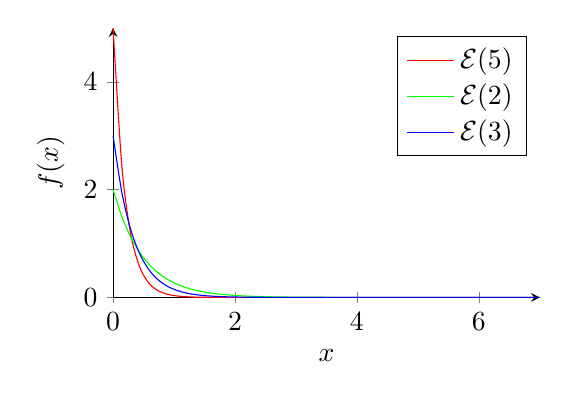
\begin{tikzpicture}
                    {
    \begin{axis}[
        domain=0:\xmax,
        axis x line=bottom, % no box around the plot, only x and y axis
        axis y line=left, % the * would suppress the arrow tips
        ylabel={$f(x)$},
        xlabel={$x$},
        legend pos=north east,
        samples=50,
        height=5cm,
        width=7cm,
        clip=false]

        \addplot[thin, smooth, red] {\lambdavala*exp(-\lambdavala*x)};
        \addlegendentry[align=left]{$\mathcal{E}(\lambdavala)$};
        \addplot[thin, smooth, green] {\lambdavalb*exp(-\lambdavalb*x)};
        \addlegendentry[align=left]{$\mathcal{E}(\lambdavalb)$};
        \addplot[thin, smooth, blue] {\lambdavalc*exp(-\lambdavalc*x)};
        \addlegendentry[align=left]{$\mathcal{E}(\lambdavalc)$};
    \end{axis}
}

                \end{tikzpicture}
                \label{fig:exponentialverteilung_a}
            }
            \subfigure[Verteilungsfunktion]{
                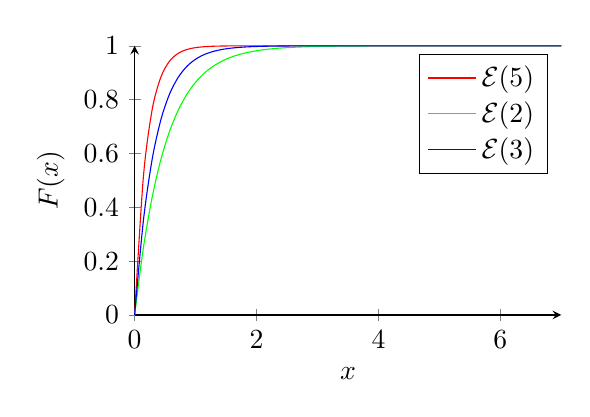
\begin{tikzpicture}
                    {
    \begin{axis}[
        domain=0:\xmax,
        axis x line=bottom, % no box around the plot, only x and y axis
        axis y line=left, % the * would suppress the arrow tips
        ylabel={$F(x)$},
        xlabel={$x$},
        legend pos=north east,
        samples=50,
        height=5cm,
        width=7cm,
        clip=false]

        \addplot[thin, smooth, red] {1-exp(-\lambdavala*x)};
        \addlegendentry[align=left]{$\mathcal{E}(\lambdavala)$};
        \addplot[thin, smooth, green] {1-exp(-\lambdavalb*x)};
        \addlegendentry[align=left]{$\mathcal{E}(\lambdavalb)$};
        \addplot[thin, smooth, blue] {1-exp(-\lambdavalc*x)};
        \addlegendentry[align=left]{$\mathcal{E}(\lambdavalc)$};
    \end{axis}
}

                \end{tikzpicture}
                \label{fig:exponentialverteilung_b}
            }

            \def\lambdavala{5}
            \def\lambdavalb{2}
            \def\lambdavalc{3}
            \def\xmax{2}
            \subfigure[Dichtefunktion]{
                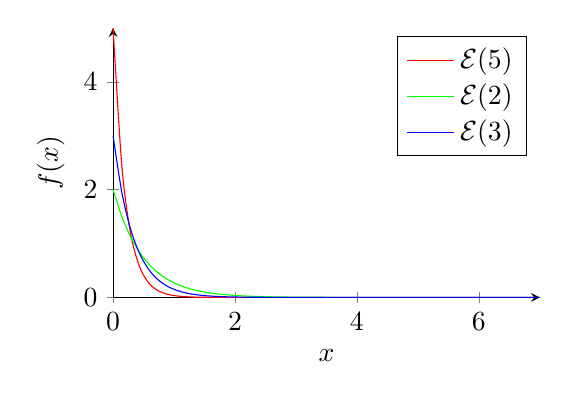
\begin{tikzpicture}
                    {
    \begin{axis}[
        domain=0:\xmax,
        axis x line=bottom, % no box around the plot, only x and y axis
        axis y line=left, % the * would suppress the arrow tips
        ylabel={$f(x)$},
        xlabel={$x$},
        legend pos=north east,
        samples=50,
        height=5cm,
        width=7cm,
        clip=false]

        \addplot[thin, smooth, red] {\lambdavala*exp(-\lambdavala*x)};
        \addlegendentry[align=left]{$\mathcal{E}(\lambdavala)$};
        \addplot[thin, smooth, green] {\lambdavalb*exp(-\lambdavalb*x)};
        \addlegendentry[align=left]{$\mathcal{E}(\lambdavalb)$};
        \addplot[thin, smooth, blue] {\lambdavalc*exp(-\lambdavalc*x)};
        \addlegendentry[align=left]{$\mathcal{E}(\lambdavalc)$};
    \end{axis}
}

                \end{tikzpicture}
                \label{fig:exponentialverteilung_a}
            }
            \subfigure[Verteilungsfunktion]{
                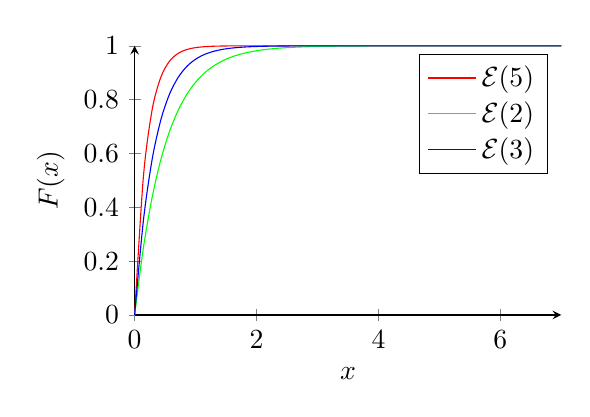
\begin{tikzpicture}
                    {
    \begin{axis}[
        domain=0:\xmax,
        axis x line=bottom, % no box around the plot, only x and y axis
        axis y line=left, % the * would suppress the arrow tips
        ylabel={$F(x)$},
        xlabel={$x$},
        legend pos=north east,
        samples=50,
        height=5cm,
        width=7cm,
        clip=false]

        \addplot[thin, smooth, red] {1-exp(-\lambdavala*x)};
        \addlegendentry[align=left]{$\mathcal{E}(\lambdavala)$};
        \addplot[thin, smooth, green] {1-exp(-\lambdavalb*x)};
        \addlegendentry[align=left]{$\mathcal{E}(\lambdavalb)$};
        \addplot[thin, smooth, blue] {1-exp(-\lambdavalc*x)};
        \addlegendentry[align=left]{$\mathcal{E}(\lambdavalc)$};
    \end{axis}
}

                \end{tikzpicture}
                \label{fig:exponentialverteilung_b}
            }
            \caption{Die Exponentialverteilung}
           \label{fig:exponentialverteilung}
        \end{figure}
    }

    Aus Abbildung \ref{fig:exponentialverteilung} kann die Wahrscheinlichkeit direkt herausgelesen
    werden (man muss nur den gelesenen Wert durch $5$ dividieren). Zum Beispiel ist die Wahrscheinlichkeit, dass zwischen den
    ersten 10 Minuten und den ersten 20 Minuten mindestens ein Anruf kommt:

    \[
    \left(1-e^{-\lambda t_{2}}\right)-\left(1-e^{-\lambda
    t_{1}}\right)=e^{-\lambda t_{1}}-e^{-\lambda
    t_{2}}=e^{-5\cdot 0.1}-e^{-5\cdot 0.2}=0,607-0,368=0,239\approx 24
    \]
    Allgemein definieren wir für die Exponentialfunktion:

    \begin{definition}
    Die Verteilung mit der Dichte $\left(\lambda >0\right)$ 
    \[
    f\left(x\right)=\begin{cases}
        \lambda e^{-\lambda x} & \textbf{falls $x\ge 0$}\\
        0 & \textbf{sonst}
        \end{cases}
    \]
    heißt Exponentialverteilung und wird mit $ExpV\left(\lambda\right)$
    notiert. Dabei ist
    \[\mathbb E\left(X\right)=\frac{1}{\lambda }\]
    \[\mathbb V\left(X\right)=\frac{1}{\lambda ^{2}}\]
    \[Med\left(X\right)=\frac{ln2}{\lambda}\]
    \end{definition}
    
    \subsection{Gammaverteilung}\index{Gammaverteilung}\index{Verteilung!Gamma-|see{Gammaverteilung}}

    \label{sec:gammaverteilung}

    Mit der Gammaverteilung (siehe Abbildung \ref{fig:gammaverteilung})ist es möglich, die Fakultät jeder positiven
    reell wertigen (im weiteren Sinne auch komplexen) Zahl zu berechnen.
    Dabei nimmt man sich das Euler'sche Integral zweiter
    Art zur Hilfe.

    {
        \def\avala{1}
        \def\lvala{2}

        \def\avalb{2}
        \def\lvalb{2}

        \def\avalc{3}
        \def\lvalc{2}

        \def\avald{1}
        \def\lvald{3}

        \def\avale{1}
        \def\lvale{1}

        \def\xmax{7}
        \begin{figure}
            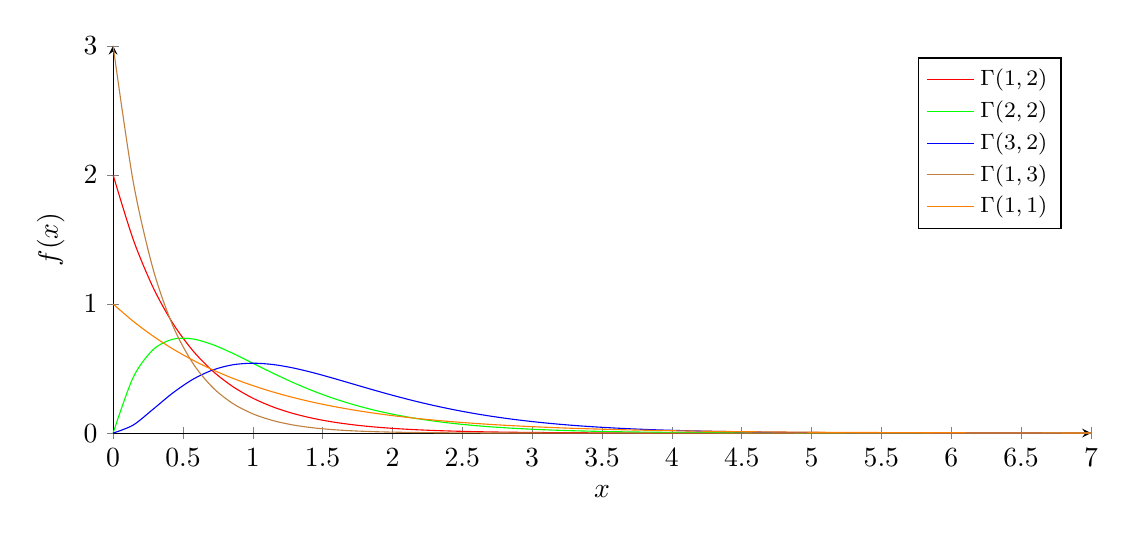
\begin{tikzpicture}
                {
    \begin{axis}[
        domain=0:\xmax,
        axis x line=bottom, % no box around the plot, only x and y axis
        axis y line=left, % the * would suppress the arrow tips
        ylabel={$f(x)$},
        xlabel={$x$},
        legend pos=north east,
        samples=50,
        height=6.5cm,
        width=14cm,
        clip=false]

        \addplot[thin, smooth, red] {\lvala^\avala/factorial(\avala-1)*x^(\avala-1)*exp(-\lvala*x)};
        \addlegendentry[align=left]{\footnotesize{$\Gamma(\avala,\lvala)$}};


        \addplot[thin, smooth, green] {\lvalb^\avalb/factorial(\avalb-1)*x^(\avalb-1)*exp(-\lvalb*x)};
        \addlegendentry[align=left]{\footnotesize{$\Gamma(\avalb,\lvalb)$}};


        \addplot[thin, smooth, blue] {\lvalc^\avalc/factorial(\avalc-1)*x^(\avalc-1)*exp(-\lvalc*x)};
        \addlegendentry[align=left]{\footnotesize{$\Gamma(\avalc,\lvalc)$}};


        \addplot[thin, smooth, brown] {\lvald^\avald/factorial(\avald-1)*x^(\avald-1)*exp(-\lvald*x)};
        \addlegendentry[align=left]{\footnotesize{$\Gamma(\avald,\lvald)$}};


        \addplot[thin, smooth, orange] {\lvale^\avale/factorial(\avale-1)*x^(\avale-1)*exp(-\lvale*x)};
        \addlegendentry[align=left]{\footnotesize{$\Gamma(\avale,\lvale)$}};

    \end{axis}
}

            \end{tikzpicture}
            \caption{Dichtefunktion der Gammaverteilung}
           \label{fig:gammaverteilung}
        \end{figure}
    }


    \begin{definition}[Gammaverteilung]:\\

    Die Gammaverteilung  $\Gamma (\alpha ,\lambda )$ ist definiert mit:

    \[f\left(x\right)=\begin{cases}
    \frac{\lambda ^{\alpha }}{\Gamma\left(\alpha \right)}
    {x^{\alpha -1}e^{-\lambda x}}&x>0\\
    0 & \text{sonst}
    \end{cases}\]
    Die \textbf{Gammafunktion} $\Gamma $\index{Gammafunktion} ist für
    beliebige  $x\in \mathbb R_{>0}$ definiert als
    \[
    \Gamma \left(x\right)=\int _{0}^{{\infty}}{t^{x-1}e^{-t}}dt
    \]
    und erfüllt die Funktionalgleichung
    \[
        \Gamma \left(x+1\right)=x\Gamma (x)\;\;\Rightarrow\;\;\Gamma(x+1)=(x)!\;\;\Rightarrow\;\; \Gamma(x)=(x-1)!
    \]
    \end{definition}

    Für die Gammafunktion gilt der Ergänzungssatz
    \[
    \Gamma \left(z\right)\Gamma \left(1-z\right)=\frac{\pi }{\sin\left(\pi z\right)}
    \]

    %TODO: add Betaverteilung
    \subsection{Cauchy-Verteilung}\index{Cauchy-Verteilung}\index{Verteilung!Cauchy-|see{Cauchyverteilung}}

    {
        \def\svala{1}
        \def\tvala{0}
        \def\svalb{0.5}
        \def\tvalb{0}
        \def\svalc{2}
        \def\tvalc{0}
        \def\svald{1}
        \def\tvald{2}

        \def\xmax{5}
        \begin{figure}
            \subfigure[Dichtefunktion]{
                \begin{tikzpicture}
                    {
    \begin{axis}[
        domain=-\xmax:\xmax,
        axis x line=bottom, % no box around the plot, only x and y axis
        axis y line=left, % the * would suppress the arrow tips
        ylabel={$f(x)$},
        xlabel={$x$},
        legend pos=north west,
        samples=50,
        height=5cm,
        width=7cm,
        clip=false]

        \addplot[thin, smooth, red] {1/pi*\svala/(\svala*\svala+(x-\tvala)*(x-\tvala))};
        \addlegendentry[align=left]{\footnotesize{$\mathcal{C}(\svala,\tvala)$}};

        \addplot[thin, smooth, green] {1/pi*\svalb/(\svalb*\svalb+(x-\tvalb)*(x-\tvalb))};
        \addlegendentry[align=left]{\footnotesize{$\mathcal{C}(\svalb,\tvalb)$}};

        \addplot[thin, smooth, blue] {1/pi*\svalc/(\svalc*\svalc+(x-\tvalc)*(x-\tvalc))};
        \addlegendentry[align=left]{\footnotesize{$\mathcal{C}(\svalc,\tvalc)$}};

        \addplot[thin, smooth, orange] {1/pi*\svald/(\svald*\svald+(x-\tvald)*(x-\tvald))};
        \addlegendentry[align=left]{\footnotesize{$\mathcal{C}(\svald,\tvald)$}};
    \end{axis}
}

                \end{tikzpicture}
                \label{fig:cauchyverteilung_a}
            }
            \subfigure[Verteilungsfunktion]{
                \begin{tikzpicture}
                    {
    \begin{axis}[
        domain=-\xmax:\xmax,
        axis x line=bottom, % no box around the plot, only x and y axis
        axis y line=left, % the * would suppress the arrow tips
        ylabel={$F(x)$},
        xlabel={$x$},
        legend pos=north west,
        samples=50,
        height=5cm,
        width=7cm,
        clip=false]

        \addplot[thin, smooth, red] {1/2+1/pi*rad(atan((x-\tvala)/\svala))};
        \addlegendentry[align=left]{\footnotesize{$\mathcal{C}(\svala,\tvala)$}};

        \addplot[thin, smooth, green] {1/2+1/pi*rad(atan((x-\tvalb)/\svalb))};
        \addlegendentry[align=left]{\footnotesize{$\mathcal{C}(\svalb,\tvalb)$}};

        \addplot[thin, smooth, blue] {1/2+1/pi*rad(atan((x-\tvalc)/\svalc))};
        \addlegendentry[align=left]{\footnotesize{$\mathcal{C}(\svalc,\tvalc)$}};

        \addplot[thin, smooth, orange] {1/2+1/pi*rad(atan((x-\tvald)/\svald))};
        \addlegendentry[align=left]{\footnotesize{$\mathcal{C}(\svald,\tvald)$}};    \end{axis}
}

                \end{tikzpicture}
                \label{fig:cauchyverteilung_b}
            }
            \caption{Die Cauchyverteilung}
           \label{fig:cauchyverteilung}
        \end{figure}
    }

    Die Cauchy-Verteilung (siehe Abbildung \ref{fig:cauchyverteilung}) wird oft verwendet, wenn man die Auswirkung von
    Ausreißern in Daten auf statistische Verfahren untersuchen möchte.
    Allgemein gilt:

    \begin{definition}[Cauchy-Verteilung]:\\
    Die Cauchy-Verteilung ist eine stetige Wahrscheinlichkeitsverteilung,
    die die Wahrscheinlichkeitsdichte
    \[
    f\left(x\right)=\frac{1}{\pi }\frac{s}{s^{2}+\left(x-t\right)^{2}}
    \]
    mit $s>0$ und $-{\infty}<t<{\infty}$ besitzt.

    Die Verteilungsfunktion der Cauchy-Verteilung ist 
    \[
    F\left(X\right)=\mathbb P\left(X<x\right)=\frac{1}{2}+\frac{1}{\pi
    }\arctan\left(\frac{x-t}{s}\right)
    \]
    \end{definition}

    \attention{Die Cauchy-Verteilung besitzt weder Erwartungswert noch Varianz.}

    Zusätzlich existiert noch eine Standard-Cauchy-Verteilung (=
    t-Verteilung) mit Zentrum $t=0$ und dem Breitenparameter $s=1$. 

    \[
    f\left(x\right)=\frac{1}{\pi (1+x^{2})}
    \]
    Es folgt ein Beweis dafür, dass kein
    Erwartungswert existiert. Man sagt, dass bei stetigen Verteilungen der
    Erwartungswert
    $\mathbb E\left(X\right)$ existiert, wenn $\int
    _{-{\infty}}^{{\infty}}{|x|f(x)}dx<{\infty}$ gilt.

    \[
    \int_{-{\infty}}^{{\infty}}{|x|\frac{1}{\pi\left(1+x^{2}\right)}}dx
    =2\int _{0}^{{\infty}}{x\frac{1}{\pi(1+x^{2})}}dx
    =\frac{1}{\pi }\int_{0}^{{\infty}}\frac{{2x}}{1+x^{2}}dx
    =\frac{1}{\pi }\ln\left(1+x^{2}\right)|_{0}^{{\infty}}
    \]
    \[
    =\frac{1}{\pi}\left({\infty}-0\right)={\infty}
    \]

    
    \subsection{Normalverteilung}\index{Normalverteilung}\index{Verteilung!Normal-|see{Normalverteilung}}
    \label{sec:normalverteilung}

    Die Gauß-Verteilung aus der Normalverteilungsfamilie gehört zu den
    theoretisch und praktisch wichtigsten Wahrscheinlichkeitsverteilungen.
    \begin{definition}
    Eine Zufallsvariable $X$ mit der Dichte
    \[
    f\left(x\right)=\frac{1}{\sqrt{2\pi }}e^{\frac{-x^{2}}{2}}
    \]
    heißt \textbf{standardnormalverteilt}\index{Standardnormalverteilung}\index{Normalverteilung!Standard-|see{Standardnormalverteilung}}\index{Verteilung!Standardnormal-|see{Standardnormalverteilung}}. Wir schreiben
    \[
    X\sim \mathcal N(0;1)
    \]
    Für Erwartungswert und Varianz gilt
    \[
    \mathbb E\left(X\right)=0
    \]
    \[
    \mathbb V\left(X\right)=1
    \]
    \end{definition}
    {
        \begin{figure}
            \def\muval{0}
            \def\sigmaval{1}
            \subfigure[Dichtefunktion]{
                \begin{tikzpicture}
                    \begin{axis}[
    domain=-4:4,
    axis x line=bottom, % no box around the plot, only x and y axis
    axis y line=left, % the * would suppress the arrow tips
    ylabel={$\varphi_{\muval,\sigmaval^2}(x)$},
    xlabel={$x$},
    ymax=1,
    legend pos=north east,
    samples=50,
    height=5cm,
    width=7cm,
    clip=false]

    \addplot[thin, smooth, blue] {normal_distribution(\muval,\sigmaval,x)};
    \addlegendentry[align=left]{$\mathcal{N}(\muval, \sigmaval)$};

    \draw [thick,dashed,black] (current axis.south-|{axis cs:\muval,0}) -- (current axis.north-|{axis cs:\muval,0}) node [above] {$\mu=\muval$};
\end{axis}

                \end{tikzpicture}
                \label{fig:standardnormalverteilung_a}
            }
            \subfigure[Verteilungsfunktion]{
                \begin{tikzpicture}
                    \begin{axis}[
    domain=-4:4,
    axis x line=bottom, % no box around the plot, only x and y axis
    axis y line=left, % the * would suppress the arrow tips
    ylabel={$\Phi_{\muval,\sigmaval^2}(x)$},
    xlabel={$x$},
    legend pos=south east,
    samples=50,
    height=5cm,
    width=7cm,
    clip=false]

    \ifnum\pdfshellescape=1 %makro to check, if shellescape is set, to prevent errors from windows
    \def\cdf(#1)(#2)(#3){1/2*(1+(erf((#3-#1)/(#2*sqrt(2)))))}
    \addplot[smooth,blue] gnuplot{1.00001*\cdf(\muval)(\sigmaval)(x)}; %multiply with 1.00001, otherwise it wouldn't be displayed
    \addlegendentry[align=left]{$\mathcal N(\muval,\sigmaval)$};
    \fi

    \draw [thick,dashed,black] (current axis.south-|{axis cs:\muval,0}) -- (current axis.north-|{axis cs:\muval,0}) node [above] {$\mu=\muval$};

\end{axis}

                \end{tikzpicture}
                \label{fig:standardnormalverteilung_b}
            }
           \caption{Die Standardnormalverteilung}
           \label{fig:standardnormalverteilung}
        \end{figure}
    }

    Oft wird die Dichte (siehe Abbildung \ref{fig:standardnormalverteilung_a}) $f\left(x\right)$ von $\mathcal N(0; 1)$ auch mit \gls{symb:varphi}, die Verteilungsfunktion (siehe Abbildung \ref{fig:standardnormalverteilung_b}) mit
\gls{symb:Phi} bezeichnet. Die Funktion $\Phi\left(x\right)$ ist tabelliert und findet sich unter Anhang \ref{tbl:standardnormalverteilung}.

    Alle Verteilungen, die aus der Standardnormalverteilung durch lineare
    Transformationen hervorgehen, bilden die Familie der
    Normalverteilungen (siehe Abbildung \ref{fig:normalverteilung})

    \begin{definition}\label{def:transformation_normalverteilung}
        Ist $X\sim\mathcal N\left(0;1\right)$ und wird $X$ \textbf{linear transformiert} \index{Standardnormalverteilung!transformation Normalverteilung}\index{Normalverteilung!transformation Standardnormalverteilung}zu
    $Y=\mu +\sigma X$ dann hat $Y$ den Erwartungswert $\mu$, die Varianz
    $\sigma^{2}$ und die Dichte 
    \[
    f_{Y}=\frac{1}{\sigma \sqrt{2\pi }}e^{\frac{-1}{2}\left(\frac{y-\mu
    }{\sigma }\right)^{2}}
    \]
    $Y$ heißt normalverteilt, geschrieben
    \[
    Y\sim\mathcal N\left(\mu ;\sigma ^{2}\right)
    \]
    \end{definition}

    {
        \begin{figure}
            \def\muvala{0}
            \def\sigmavala{1}
            \def\muvalb{0}
            \def\sigmavalb{0.5}
            \def\muvalc{0}
            \def\sigmavalc{2}

            \subfigure[Dichtefunktion]{
                \begin{tikzpicture}
                    \input{chapters/zufallsvariable/dens_norm}
                \end{tikzpicture}
                \label{fig:normalverteilung_a}
            }
            \subfigure[Verteilungsfunktion]{
                \begin{tikzpicture}
                    \input{chapters/zufallsvariable/dist_norm}
                \end{tikzpicture}
                \label{fig:normalverteilung_b}
            }

            \def\muvala{0}
            \def\sigmavala{1}
            \def\muvalb{-2}
            \def\sigmavalb{1}
            \def\muvalc{2}
            \def\sigmavalc{1}
            \subfigure[Dichtefunktion]{
                \begin{tikzpicture}
                    \begin{axis}[
    domain=-4:4,
    axis x line=bottom, % no box around the plot, only x and y axis
    axis y line=left, % the * would suppress the arrow tips
    ylabel={$\varphi_{\mu,\sigma}(x)$},
    xlabel={$x$},
    ymax=1,
    legend pos=north east,
    samples=50,
    height=5cm,
    width=7cm,
    clip=false]

    \addplot[thin, smooth, blue] {normal_distribution(\muvala,\sigmavala,x)};
    \addlegendentry[align=left]{\footnotesize{$\mathcal{N}(\muvala, \sigmavala)$}};

    \addplot[thin, smooth, green] {normal_distribution(\muvalb,\sigmavalb,x)};
    \addlegendentry[align=left]{\footnotesize{$\mathcal{N}(\muvalb, \sigmavalb)$}};

    \addplot[thin, smooth, red] {normal_distribution(\muvalc,\sigmavalc,x)};
    \addlegendentry[align=left]{\footnotesize{$\mathcal{N}(\muvalc, \sigmavalc)$}};

\draw [thick,dashed,black] (current axis.south-|{axis cs:\muvala,0}) -- (current axis.north-|{axis cs:\muvala,0}) node [above] {\footnotesize{$\mu_1=\muvala$}};
\draw [thick,dashed,black] (current axis.south-|{axis cs:\muvalb,0}) -- (current axis.north-|{axis cs:\muvalb,0}) node [above] {\footnotesize{$\mu_2=\muvalb$}};
\draw [thick,dashed,black] (current axis.south-|{axis cs:\muvalc,0}) -- (current axis.north-|{axis cs:\muvalc,0}) node [above] {\footnotesize{$\mu_3=\muvalc$}};

\end{axis}

                \end{tikzpicture}
                \label{fig:normalverteilung_c}
            }
            \subfigure[Verteilungsfunktion]{
                \begin{tikzpicture}
                    \input{chapters/zufallsvariable/dist_norm_b}
                \end{tikzpicture}
                \label{fig:normalverteilung_d}
            }
           \caption{Die Normalverteilung}
           \label{fig:normalverteilung}
        \end{figure}
    }

    \index{Stetige Verteilung|)}

    \section{Verteilungen Zusammenfassung}\index{Verteilung!Zusammenfassung}
    \textbf{Diskrete Verteilungen}\\
    \begin{tabular}{|l|l|c|c|c|}\hline
    Name & Symbol & $p(x)$ & $\mathbb E(X)$ & $\mathbb V(X)$ \\\hline
    Binomial\index{Binomialverteilung}\label{diskrete_verteilung:binomial} & $\mathcal B(n,p)$ & ${n\choose x}p^x(1-p)^{n-x} (0\le x\le n)$& $np$ & $np(1-p)$ \\\hline
    Gleichverteilung\index{Gleichverteilung} & $\mathcal D(a,b)$& ${1\over b-a+1} (a\le x\le b)$ & ${a+b\over 2}$&
    ${(b-a)^2-1\over 12}$ \\\hline
    Geometrisch\index{Geometrische Verteilung}\label{diskrete_verteilung:geometrisch} & $\mathcal G(p)$ & $p(1-p)^x, (x\ge 0)$ & ${1-p\over p}$ & ${1-p\over p^2}$
    \\\hline
    Poisson\index{Poissonverteilung}& $\mathcal P(\lambda)$ & ${\lambda^xe^{-\lambda}\over x!}$ & $\lambda$
    & $\lambda$ \\\hline
    Hypergeometrisch\index{Hypergeometrische Verteilung} & $\mathcal H(N,A,n)$
    & ${{A\choose x}{N-A\choose n-x}\over {N\choose n}} (0\le x\le n)$ &
    $nA\over N$ & $ nA(N-A)(N-n)\over N(N-1)$\\\hline
    \end{tabular}

    \textbf{Stetige Verteilungen}\\
    \begin{tabular}{|l|l|c|c|c|}\hline
    Name & Symbol & $f(x)$ & $\mathbb E(X)$ & $\mathbb V(X)$ \\\hline
    Gleichverteilung\index{Gleichverteilung} & $\mathcal U(a,b)$ & ${1\over b-a} (a\le x\le b)$ & $a+b\over 2$ &
    $(b-a)^2\over 12$\\\hline
    Exponential\index{Exponentialverteilung} & $\mathcal E(\lambda)$ & $\lambda e^{-\lambda x} (x\ge 0)$ & $1\over\lambda$ & $1\over\lambda^2$ \\\hline
    Gamma\label{stetige_verteilung:gamma}\index{Gammaverteilung} & $\Gamma(\alpha,\lambda)$ &
    ${\lambda^\alpha x^{\alpha-1}\over\Gamma(\alpha)}e^{-\lambda x} (x|\ge 0)$ &
    $\alpha\over\lambda$ & $\alpha\over\lambda^2$\\\hline
    Cauchy\index{Cauchyverteilung} & $\mathcal C(a)$ & ${a\over\pi(x^2+a^2)}$ & N.A. & N.A.\\\hline
    Normal\index{Normalverteilung}\label{stetige_verteilung:normal}& $\mathcal N(\mu,\sigma^2)$ & ${1\over\sqrt{2\pi\sigma^2}}
    \exp(-{(x-\mu)^2\over 2\sigma^2})$ & $\mu$ & $\sigma^2$\\\hline
    Beta 1.\ Art\label{sec:betaverteilung_first}\label{stetige_verteilung:beta_first}\index{Betaverteilung (1.Art)}&$\beta_1(\alpha,\lambda)$&${x^{\alpha-1}
    (1-x)^{\beta-1}\over B(\alpha,\beta)}
     (0\le x\le 1)$&${\alpha\over\alpha+\beta}$&
    ${\alpha\beta\over(\alpha+\beta+1)(\alpha+\beta)^2}$\\\hline
    Beta 2.\ Art\index{Betaverteilung (2.Art)}&$\beta_1(\alpha,\lambda)$&${x^{\alpha-1}
    (1+x)^{-\alpha-\beta}\over B(\alpha,\beta)}
     (0\le x)$&${\alpha\over\beta-1} (\beta>1)$&
    ${\alpha(\alpha+\beta-1)\over(\beta-2)(\beta-1)^2}(\beta>2)$\\\hline
    \end{tabular}

    

    \index{Zufallsvariable|)}
}
